\chapter{Business Processes}
In this chapter we analyze a set of business processes which are
fundamental activities inside our organization, we provide an analysis of
these processes and the results of a simulation.
 
Before going in deeper details in analyzing the processes is useful to get
a wider view on the organization structure.
AllSpark, is an enterprise with the aim to develop and deploy services in
the IT area.
 
Our products can vary from a common web hosting service to very complex and
possibly innovative security systems, and therefore we need to distinguish
the different departments in which our organization is divided.
 
\section{Departments and structure}
AllSpark organization is divided in several activity areas, each one of them
contains the processes and the people needed to operate in a specific
field.
 
For a more detailed view on the organization is useful to provide a
formalization of these concepts, through a set of diagrams which are going
to be described in the following sections. In particular the attention has
been focused in representing the two sides of the organization: first it's
possible to analyze which are the different roles inside the company and
how they are distributed, then is presented a view on which business
processes are involved in the different areas of the company.
 
\subsection{Working structure}
The working structure represent the general structure of AllSpark internal
organization. For simplicity the number of employees is not represented
since there may be several entities for each "Performer" depending on the
working load and on the size of the projects involved. Each performer is a
facet entity since several people may collaborate in that position to reach
the Roles defined, but identifying all of them with a single term and
element in the structure, permits a simpler representation of the concept.
 
The two main areas, Administrative and Research and Development, distinguish
the scope the employee would reach. In the former the main interest is
directly connected to the set of functions which permits the right and
complete Company lifecycle. The latter is bind to the Company productivity,
that are the basic elements which are involved in the growing of
the invoice.
 
The Working Team is an abstract organizational unit which represent a group
of employee which are involved in a particular project, or in some some
cases in different ones, that need different skills and knowledges to be
developed. In the organization there may be several Working Team in order to
maximize the performance in productivity and in the Project management.
 
The Public Relation organizational unit aims to represent the group of
people who are charged to represent the Company in meetings, in the
approaching with customers and for consulting.
 
Figure \ref{2img:working} can describe in details how people working for
AllSpark is organized inside the company.
 
\begin{figure}
\begin{centering}
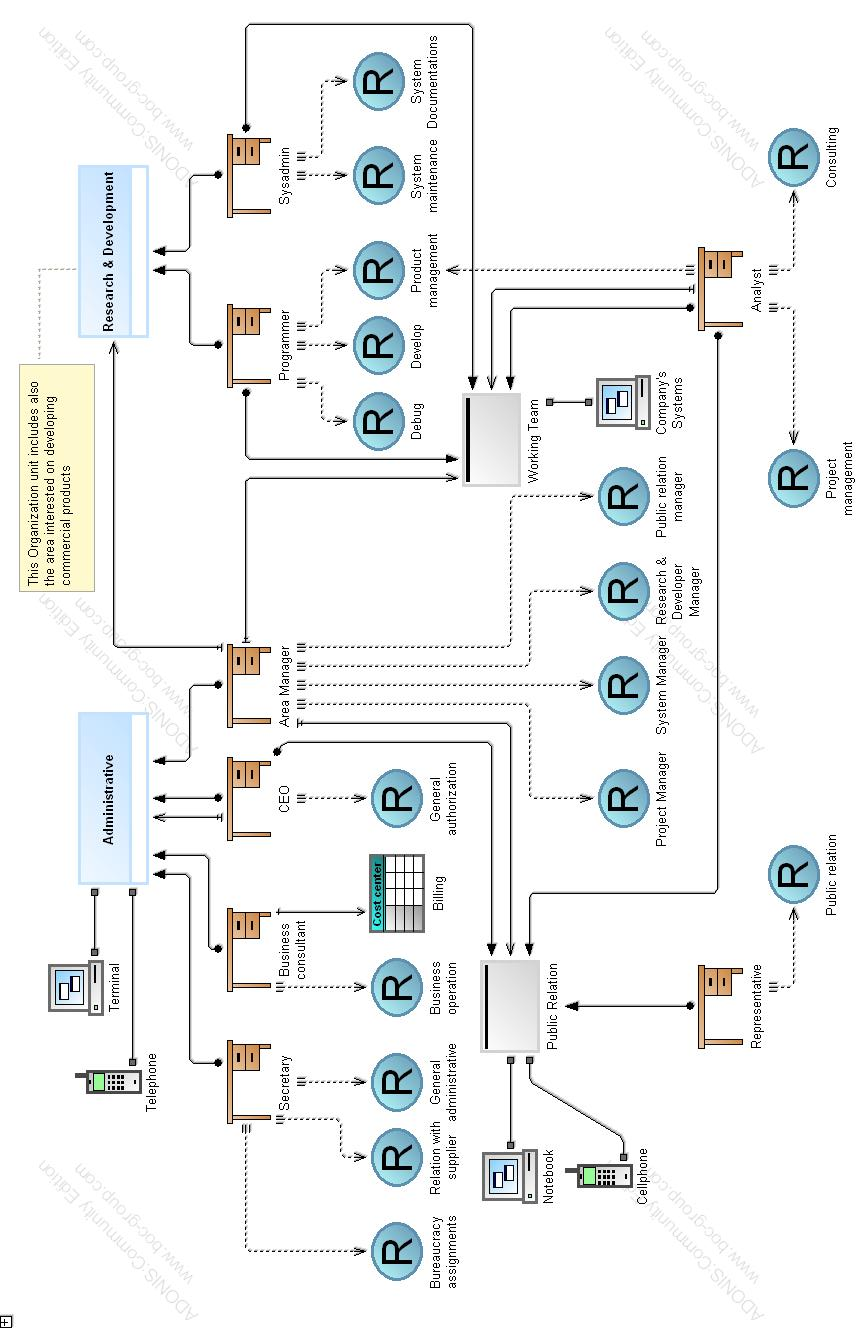
\includegraphics[scale=0.45]{assign2/adonis/imgs/working_structure.jpg}
\caption{AllSpark working structure}
\label{2img:working}
\end{centering}
\end{figure}
 
\subsection{Company organization}
In the AllSpark organization is possible to identify the following
different areas:
\begin{description}
\item[Administration:] This part of the enterprise manages the
administrative part of the organization, takes marketing decision, follows
the public relations with external partners, solves bureaucratic issues
and is responsible for the financial operations.
\item[Project Management:] This segment of the organization is involved in
the core processes of manage the different phases of project development.
These activities represent a set of core functions in the organizations
aims, is this sector, in facts, which is responsible for the actual
implementation of our products.
\item[Working resource management:] The processes and resources which are
involved in this sector provide support for the maintenance of hardware
and software. There are processes dedicated to reparation as to the update
of different resources.
\item[Course and Certification:] AllSpark, as an enterprise, organizes
courses for developers and sysadmins. For this reason a particular division
of the organization is dedicated to the management of courses and seminars.
\item[Research and Development:] The employees in this area work actively in
the research's world, mainly in security related field. In our organization
this section is vital for improving our products and develop new one.
\end{description}
 
The company map in figure \ref{2img:cmap} depicts clearly the business processes
performed in each section and how them are related to each other.
 
\begin{figure}
\begin{centering}
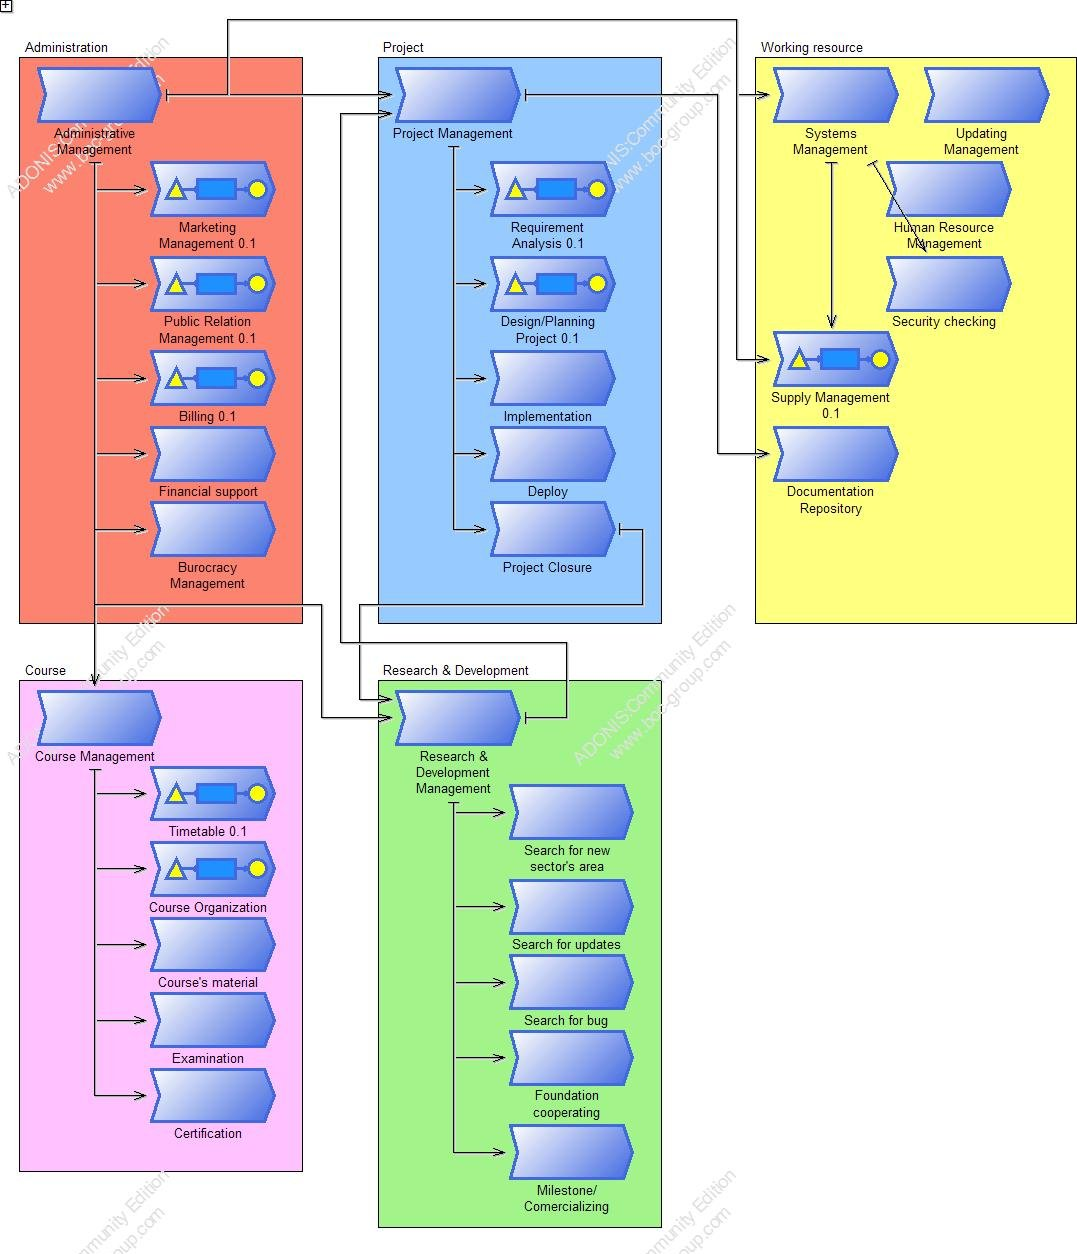
\includegraphics[scale=0.43]{assign2/adonis/imgs/companymap.jpg}
\caption{AllSpark company map}
\label{2img:cmap}
\end{centering}
\end{figure}
 
\subsection{Login}

\begin{figure}
\begin{centering}
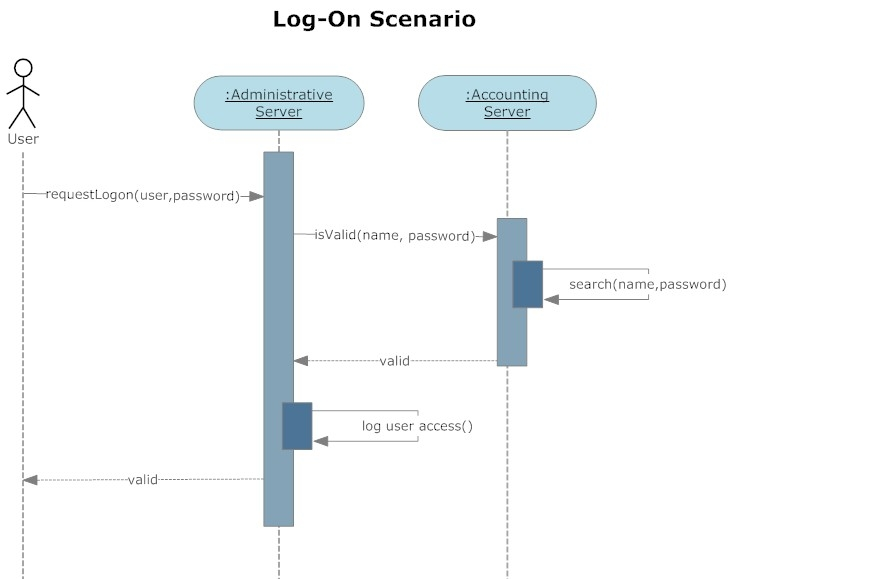
\includegraphics[scale=0.45]{assign3/sdraw/imgs/login.jpg}
\caption{Login sequence diagram.}
\label{3img:[sequence]login}
\end{centering}
\end{figure}

\subsection{Sending order}
\begin{figure}
\begin{centering}
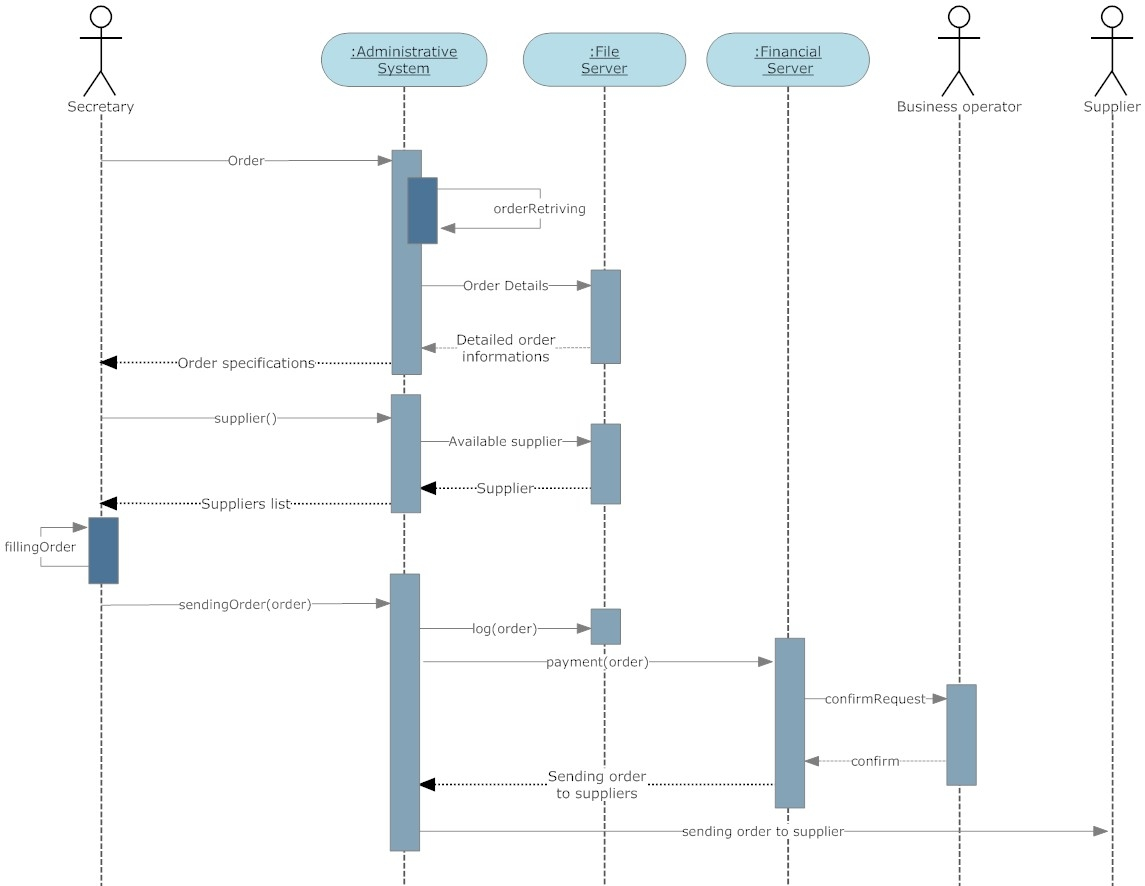
\includegraphics[scale=0.45,angle=90]{assign3/sdraw/imgs/sending_order.jpg}
\caption{Sending order sequence diagram.}
\label{3img:[sequence]sending_order}
\end{centering}
\end{figure}

\subsection{Maintenance schedule}
\begin{figure}
\begin{centering}
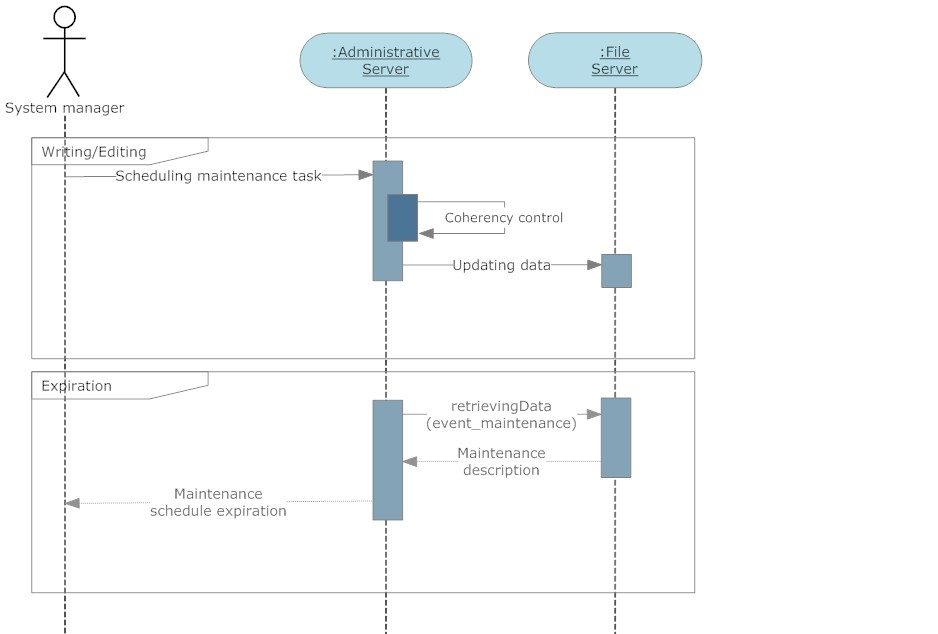
\includegraphics[scale=0.50]{assign3/sdraw/imgs/maintenance.jpg}
\caption{Maintenance schedule sequence diagram.}
\label{3img:[sequence]maintenance}
\end{centering}
\end{figure}

\subsection{Meeting management}
\begin{figure}
\begin{centering}
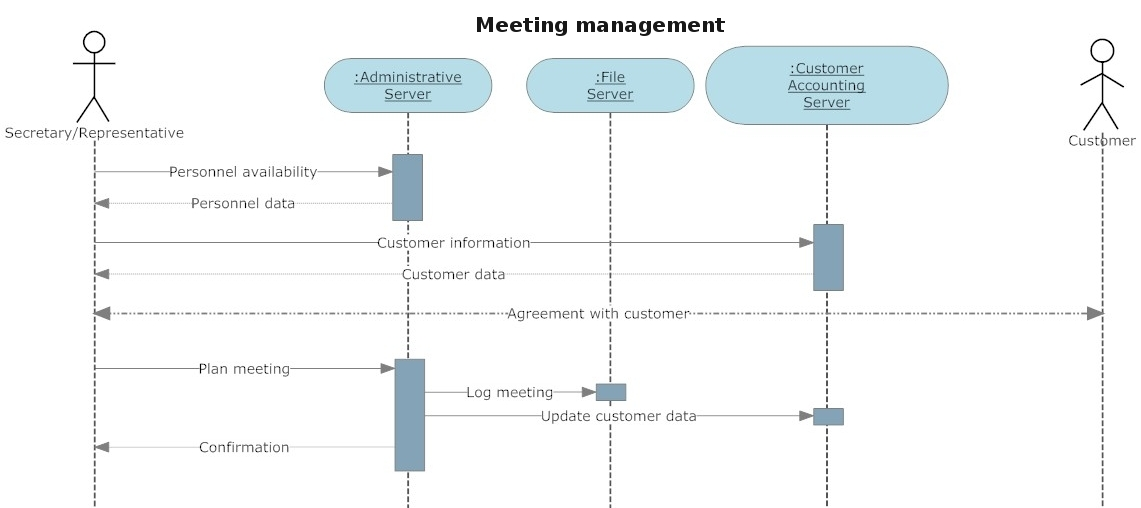
\includegraphics[scale=0.35]{assign3/sdraw/imgs/meeting.jpg}
\caption{Meeting management sequence diagram.}
\label{3img:[sequence]meeting}
\end{centering}
\end{figure}

\subsection{Project planning}
\begin{figure}
\begin{centering}
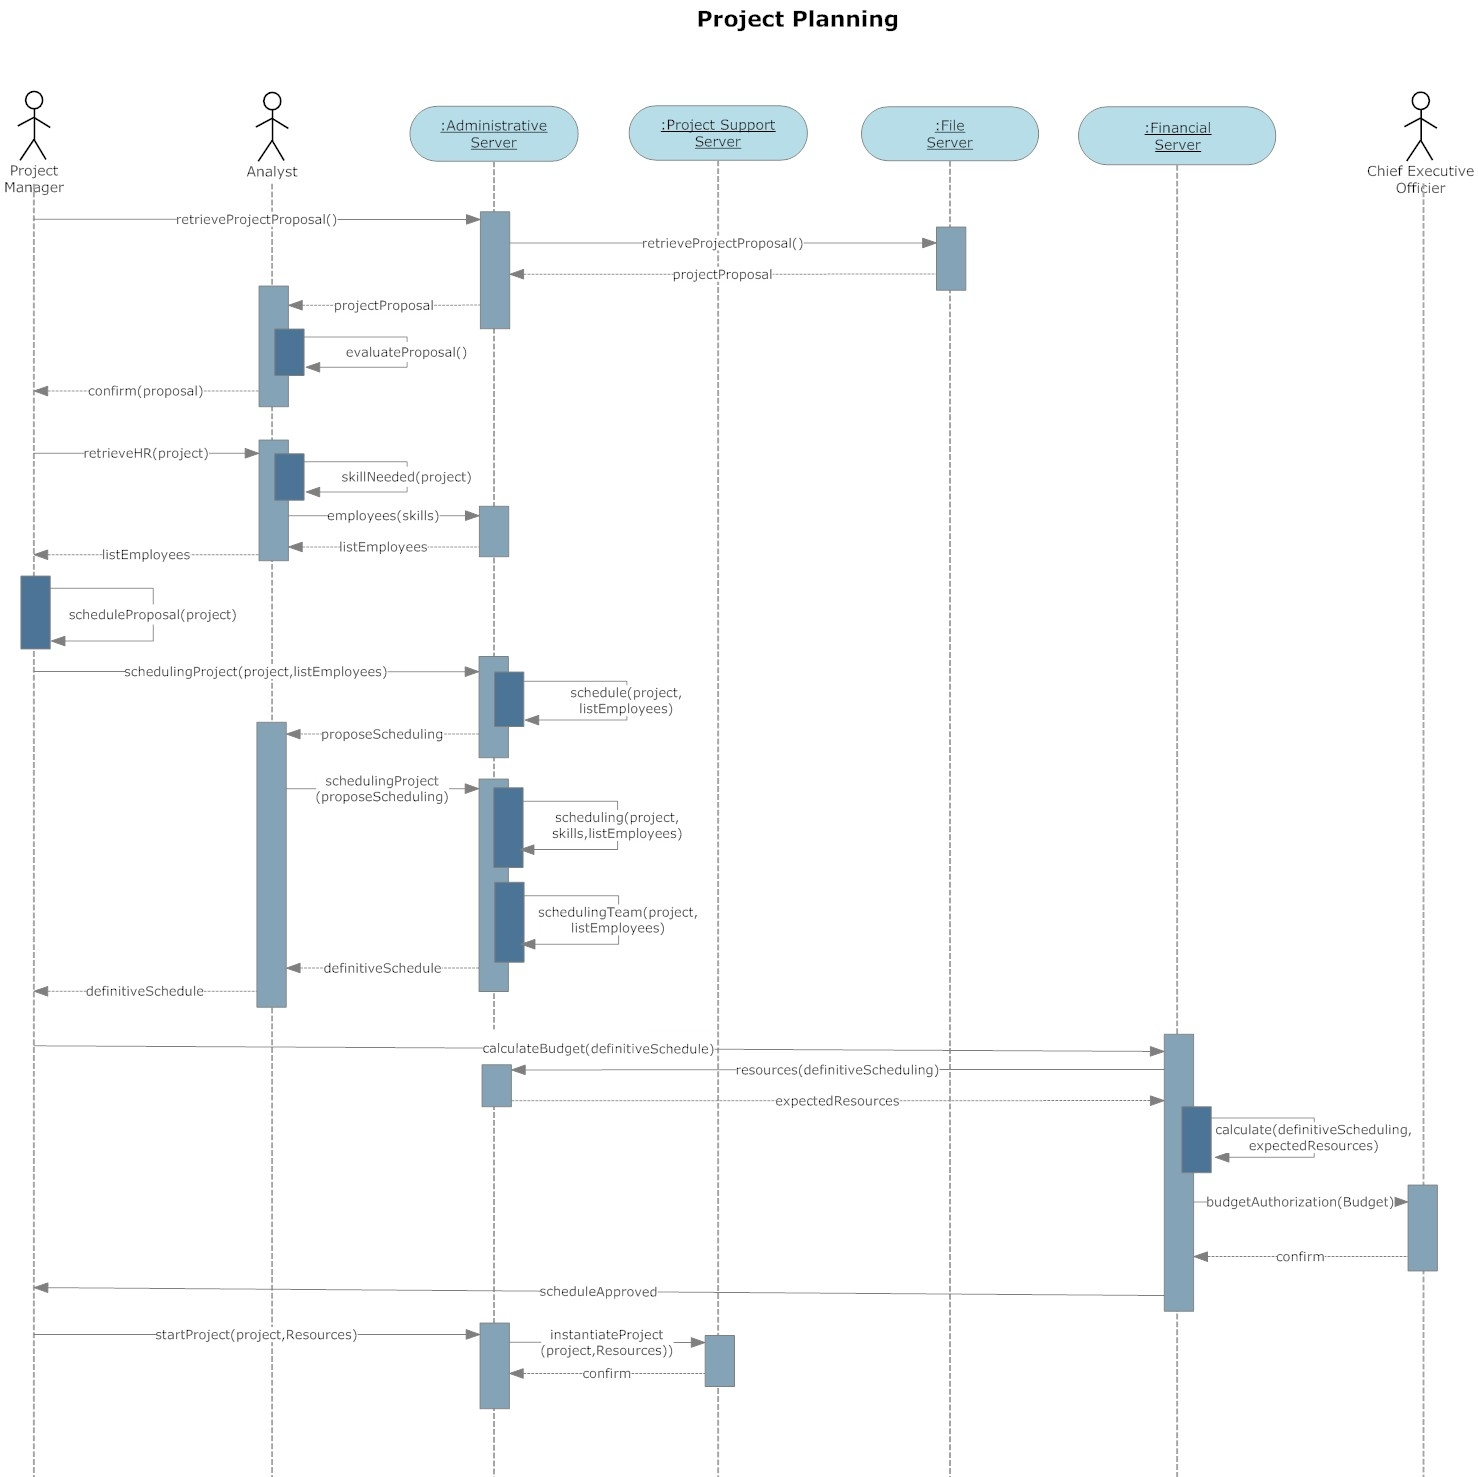
\includegraphics[scale=0.30,angle=90]{assign3/sdraw/imgs/project_planning.jpg}
\caption{Project planning sequence diagram.}
\label{3img:[sequence]project_planning}
\end{centering}
\end{figure}

\subsection{Checking work}
\begin{figure}
\begin{centering}
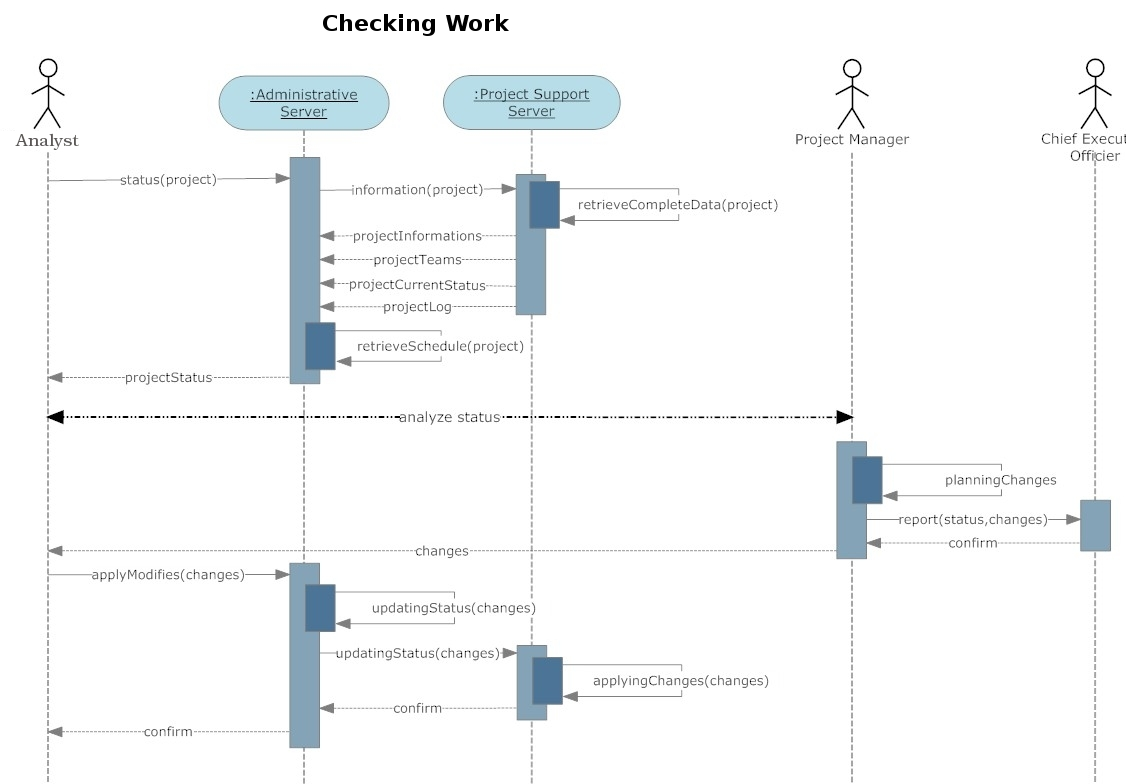
\includegraphics[scale=0.35]{assign3/sdraw/imgs/checking.jpg}
\caption{Checking work sequence diagram.}
\label{3img:[sequence]checking}
\end{centering}
\end{figure}

\subsection{Team monitoring}
\begin{figure}
\begin{centering}
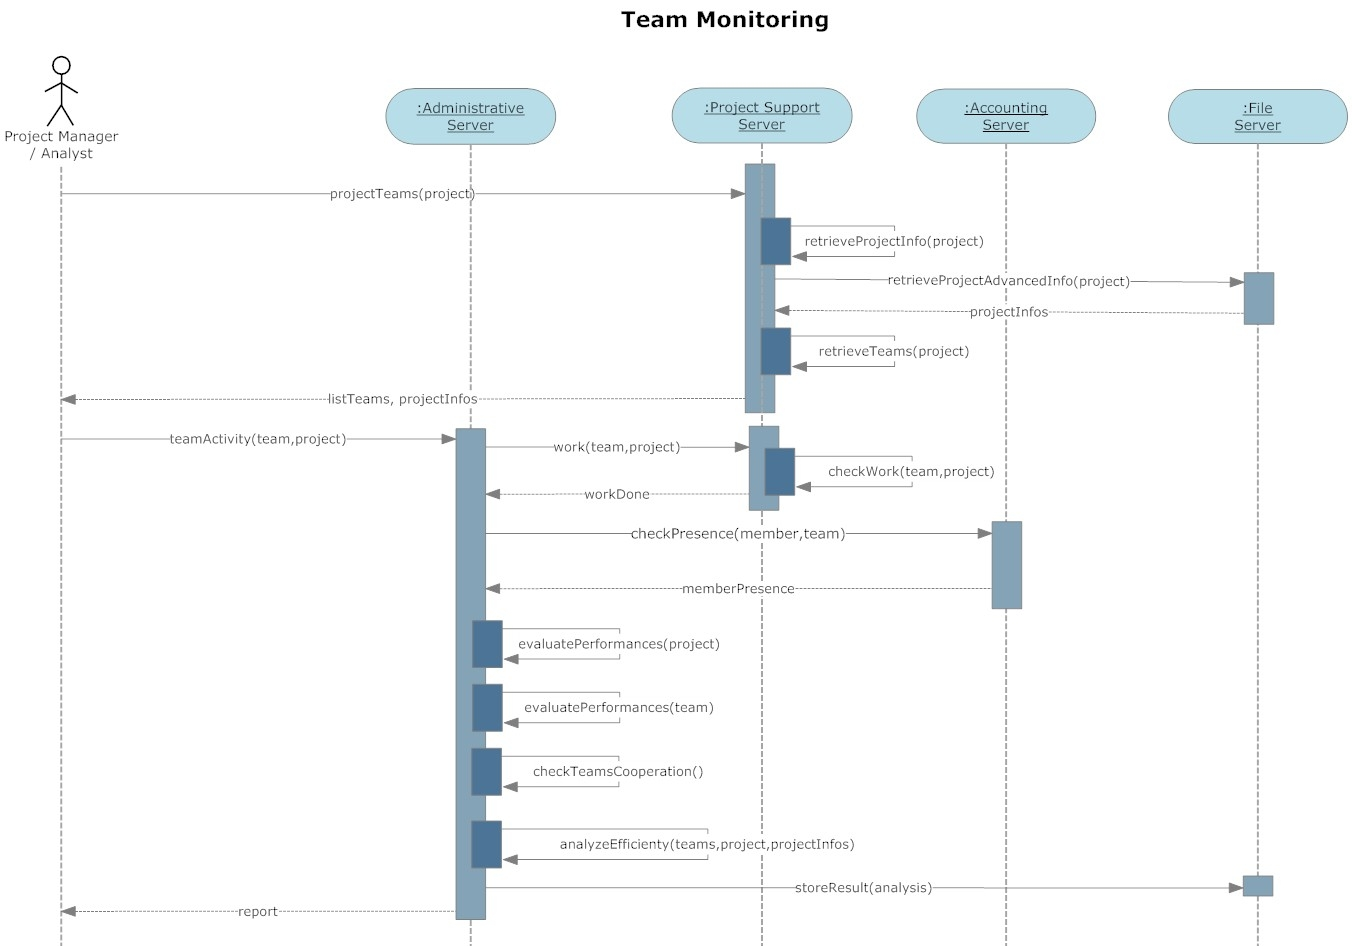
\includegraphics[scale=0.40,angle=90]{assign3/sdraw/imgs/team_monitoring.jpg}
\caption{Team monitoring sequence diagram.}
\label{3img:[sequence]team_monitoring}
\end{centering}
\end{figure}

\subsection{Course log}
\begin{figure}
\begin{centering}
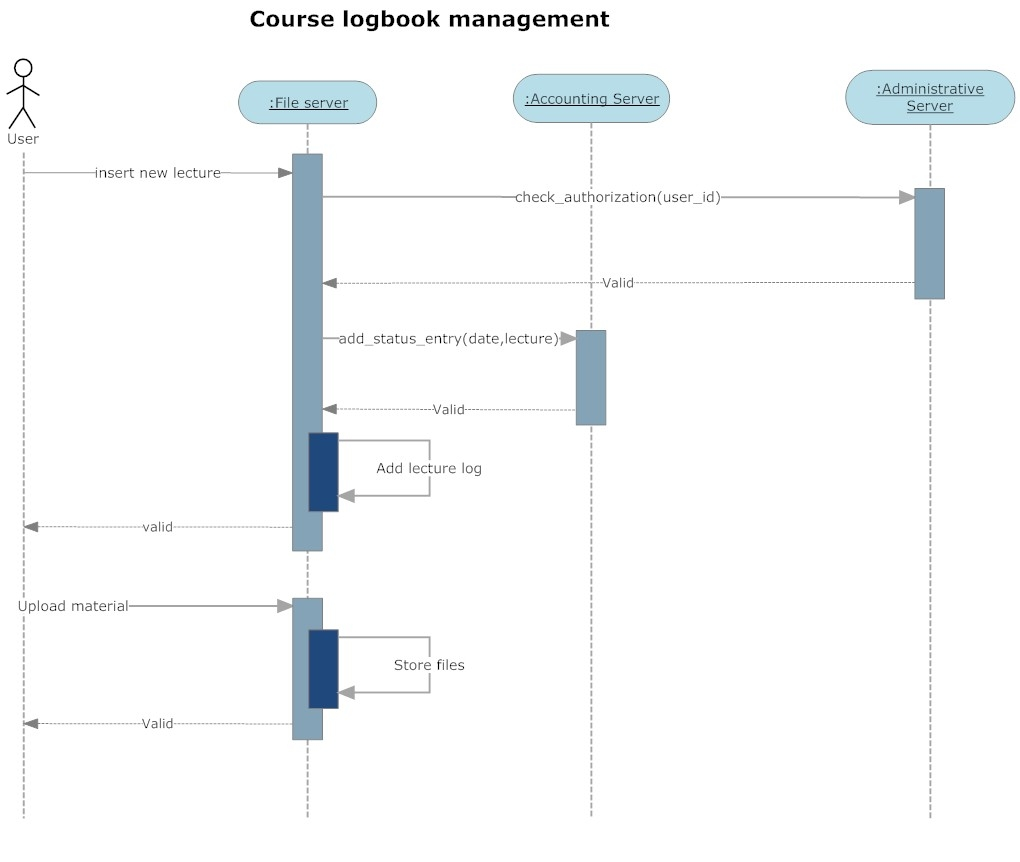
\includegraphics[scale=0.45]{assign3/sdraw/imgs/course_log.jpg}
\caption{Course log sequence diagram.}
\label{3img:[sequence]course_log}
\end{centering}
\end{figure}

\subsection{Certification}
\begin{figure}
\begin{centering}
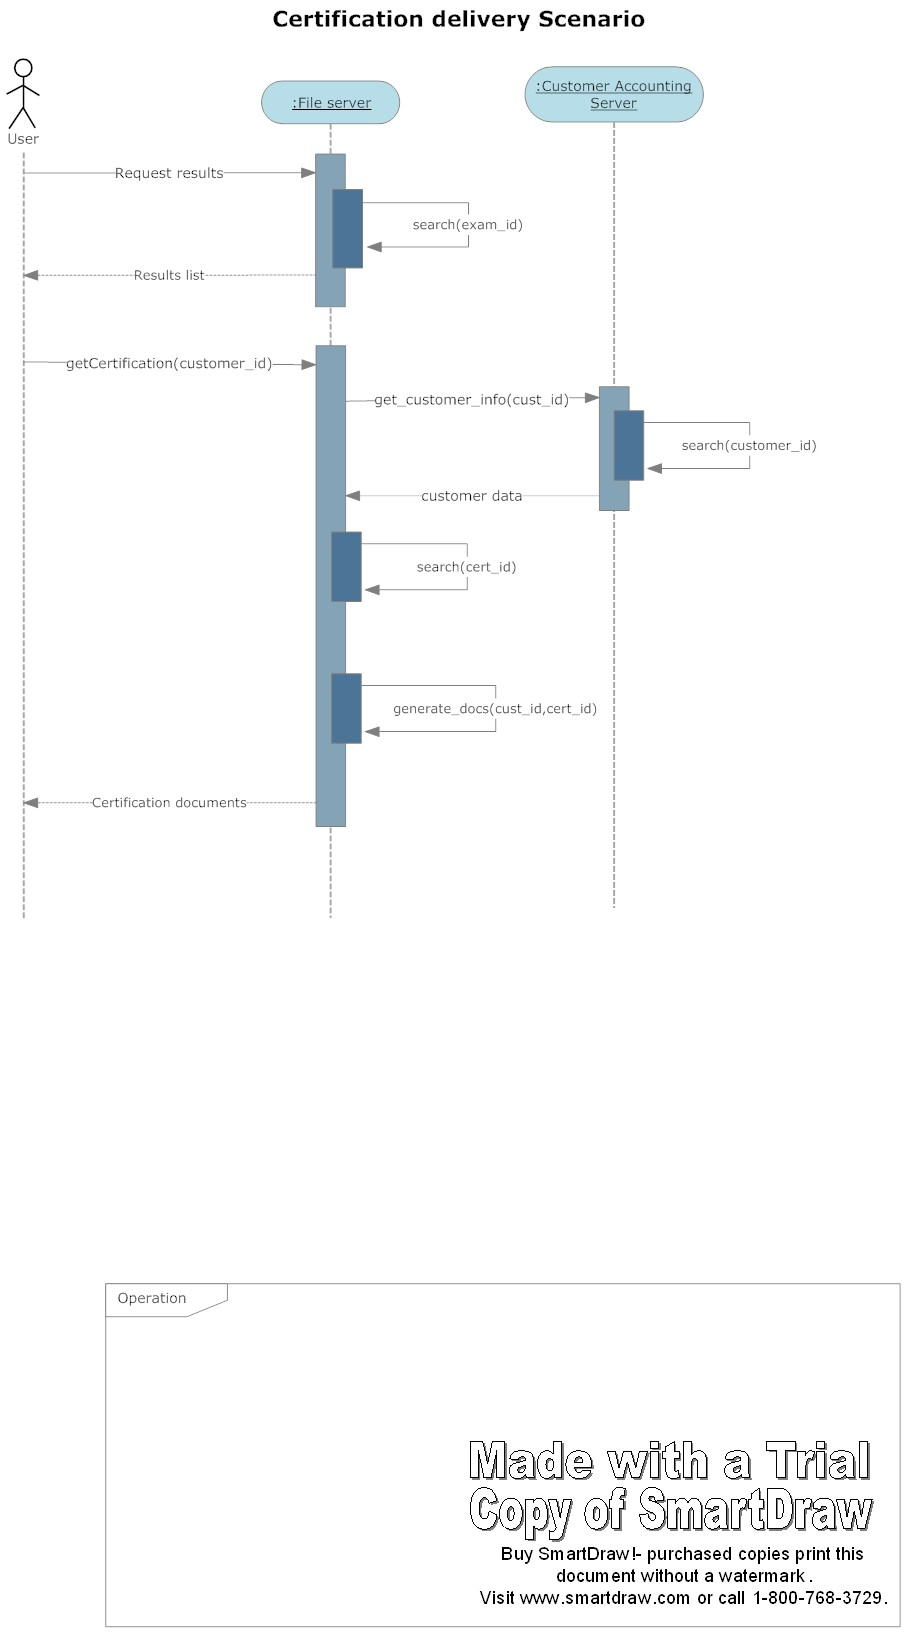
\includegraphics[scale=0.55]{assign3/sdraw/imgs/certification.jpg}
\caption{Certification sequence diagram.}
\label{3img:[sequence]certification}
\end{centering}
\end{figure}

\subsection{Campaign planning}
\begin{figure}
\begin{centering}
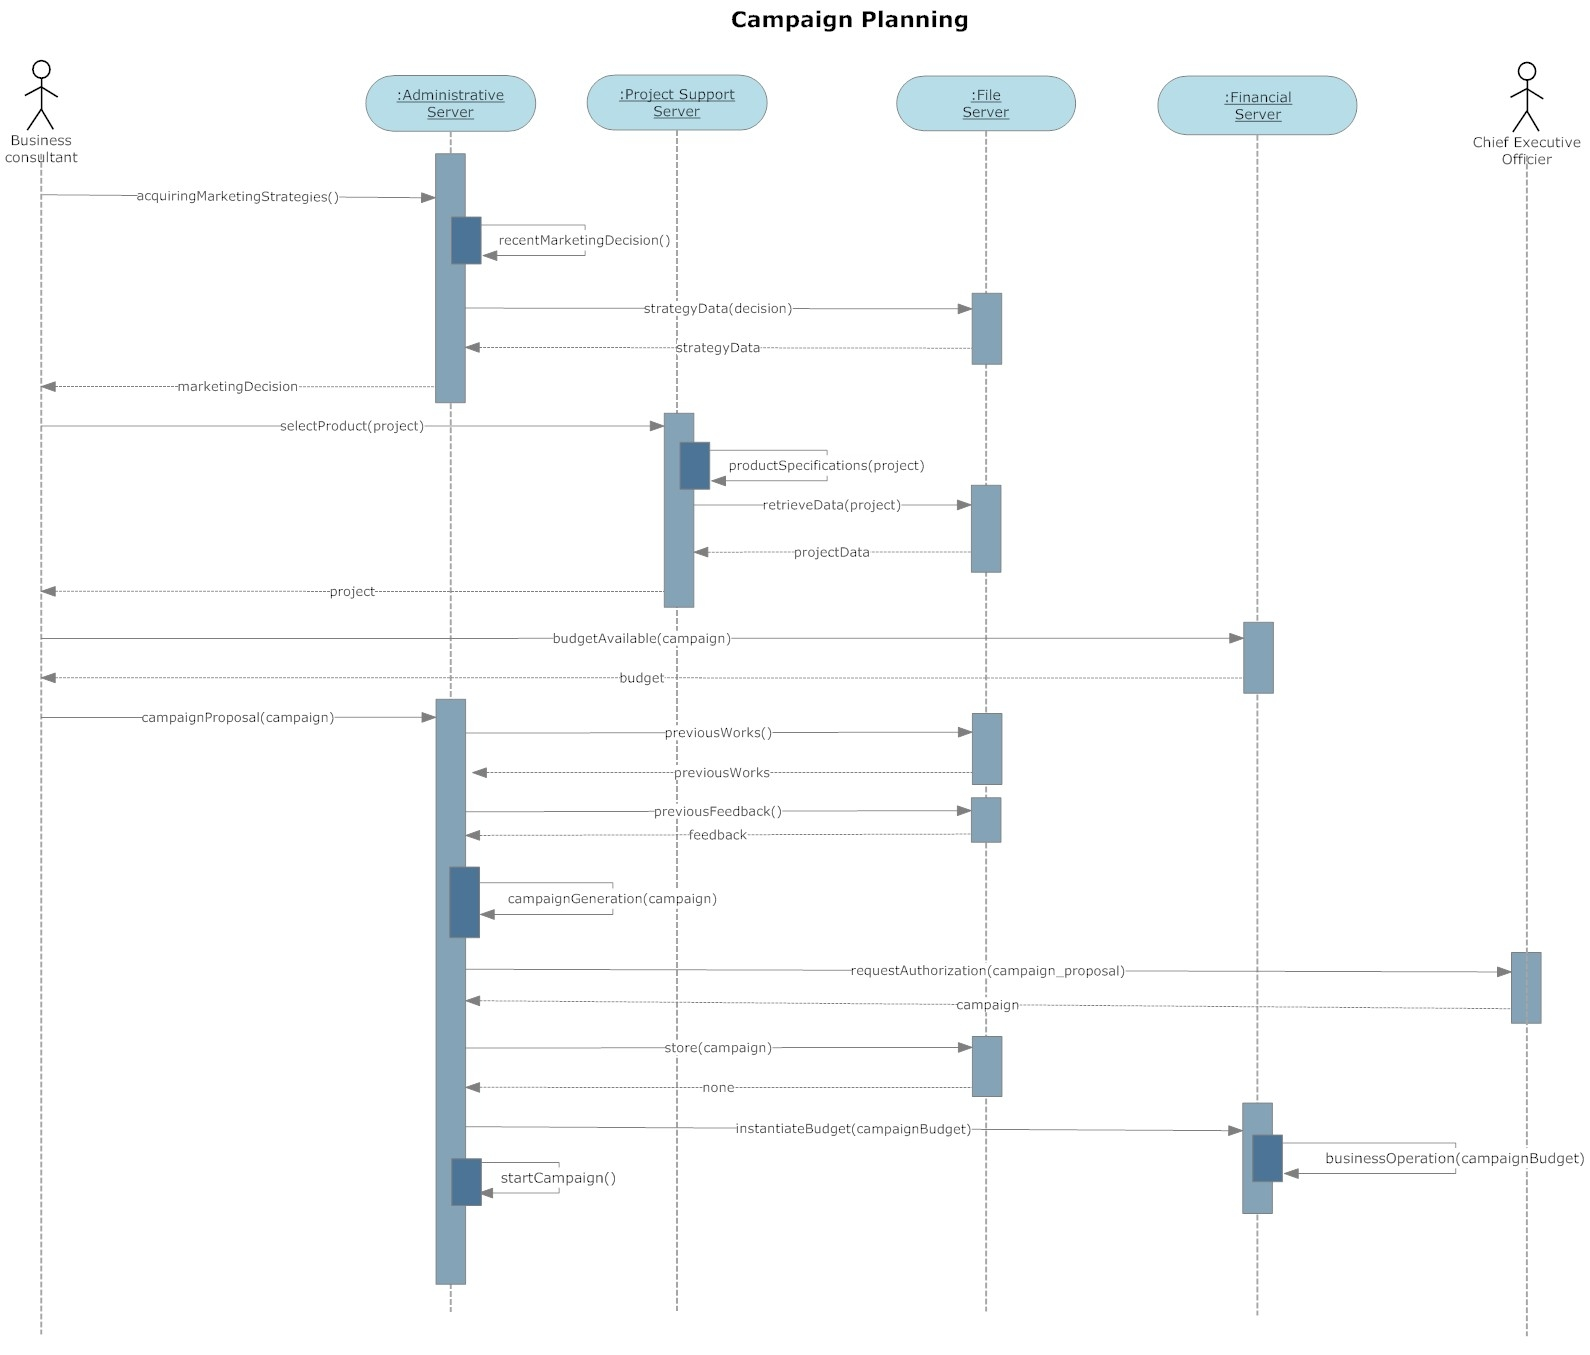
\includegraphics[scale=0.35,angle=90]{assign3/sdraw/imgs/campaign_planning.jpg}
\caption{Campaign planning sequence diagram.}
\label{3img:[sequence]campaign_planning}
\end{centering}
\end{figure}

\subsection{Inventory management}
\begin{figure}
\begin{centering}
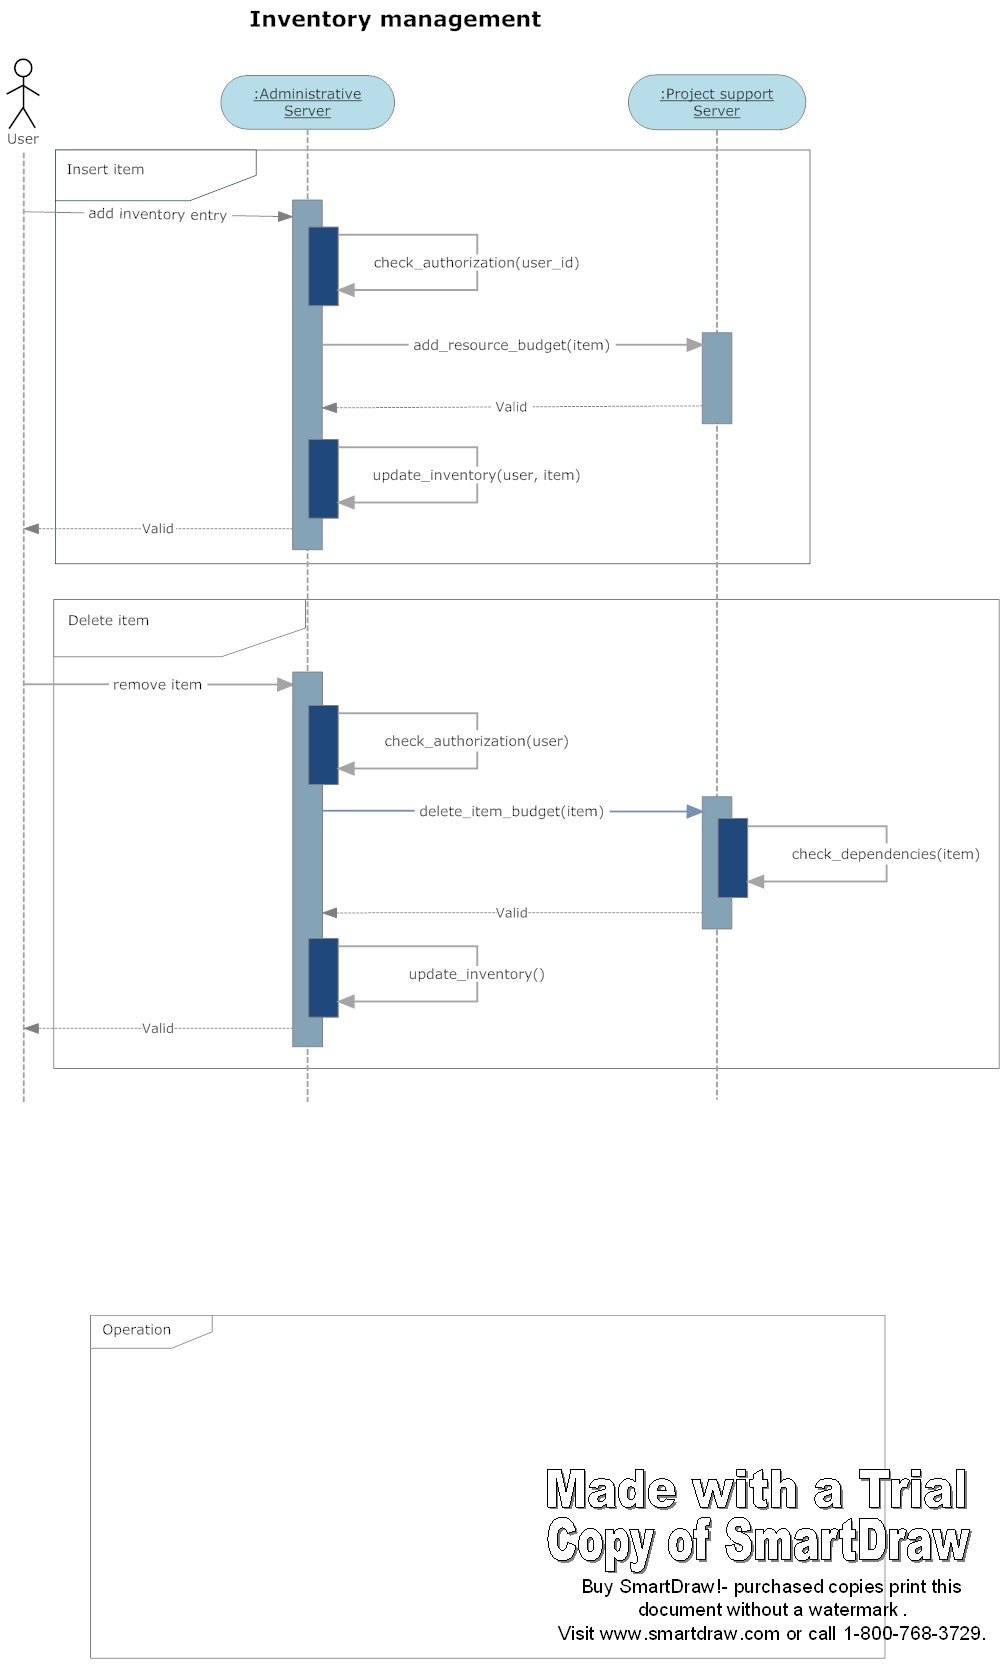
\includegraphics[scale=0.45]{assign3/sdraw/imgs/inventory.jpg}
\caption{Inventory management sequence diagram.}
\label{3img:[sequence]inventory}
\end{centering}
\end{figure}

\subsection{Editing documentation}
\begin{figure}
\begin{centering}
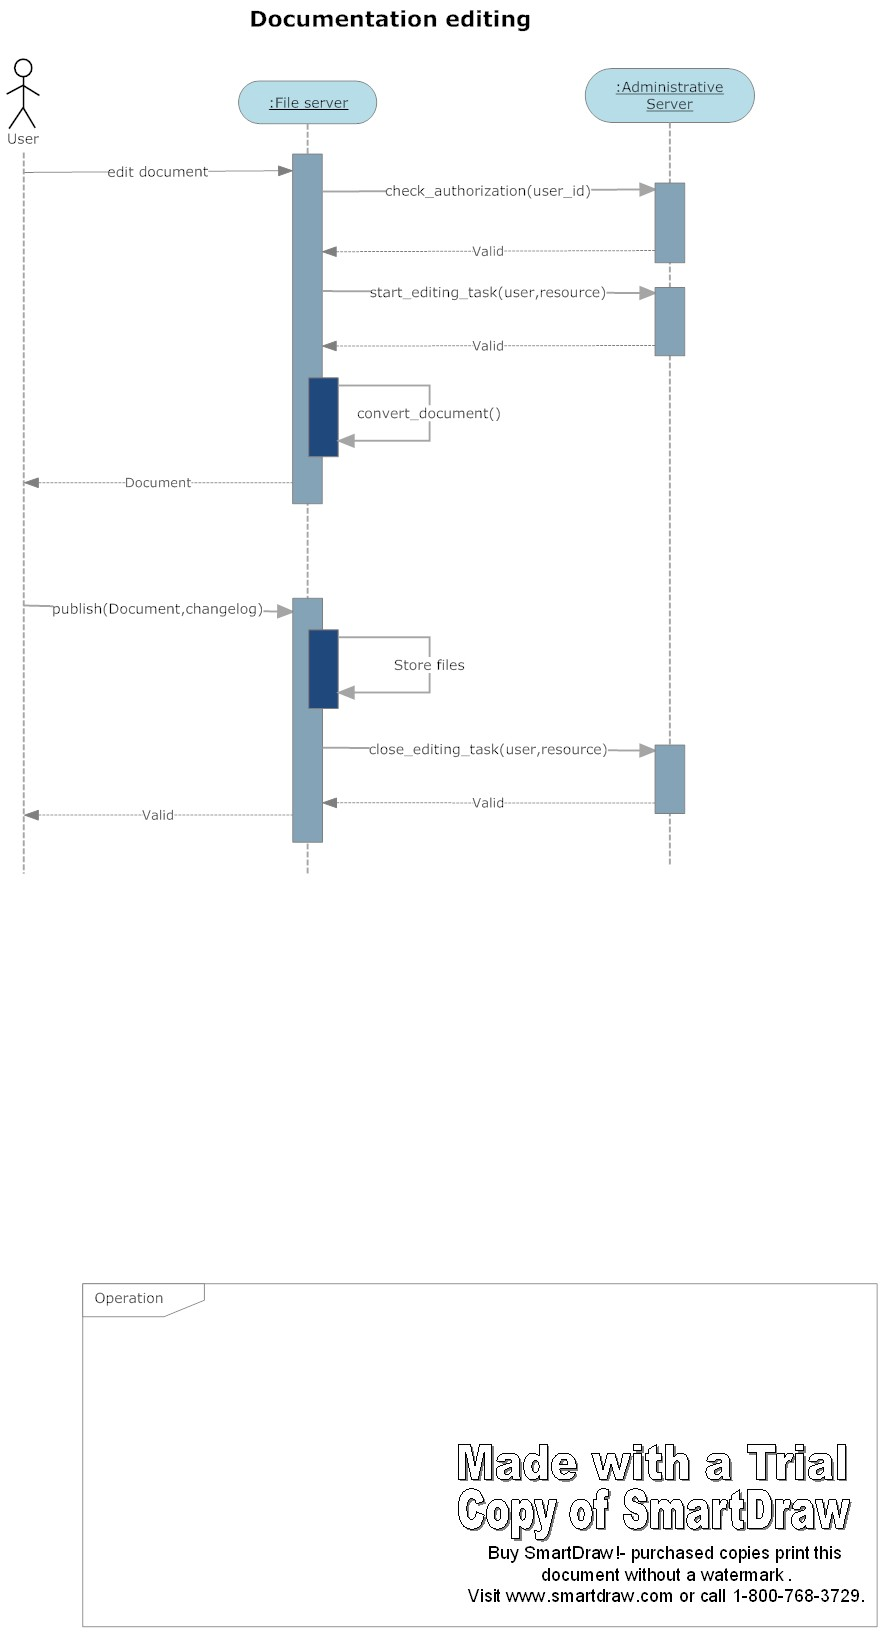
\includegraphics[scale=0.45]{assign3/sdraw/imgs/editing.jpg}
\caption{Editing documentation sequence diagram.}
\label{3img:[sequence]editing}
\end{centering}
\end{figure}
\section{Working Resources Area}
The Working Resource Area encompass all the AllSpark's business processes that characterize its right lifecycle and functionalities releated to the working environment. Each business process aims to satisfy some specific objective needed by correctness and the efficiency of processes in other areas, but that are not required in advance for the productivity roles the Company wants to achieve. The employees involved in the business processes are potentially of all kind foreseen in the Working Structure presented in figure \ref{2img:working}.

A particular observation is reserved to the responsibility role of this Area. Since each area has a responsible the discussion about it is relavant, but not so simple to define a unique responsible except for the CEO; generally is defined an Area Manager that leads all the business processes, but pratically is more efficient that each process is assigned to the most similar manager.

The business process Systems management has not been modeled since is very general and most of its processes are not really interesting.

\subsection{Updating Management}
This Updating Management business process is derived by the macro business process ``Systems Management'' that provides, as the name suggests, the service of ``up to date'' systems meaning softwares, both products and tools, and hardwares in order to minimize the presence of bugs, improve the efficiency and acquire new features.

The main responsible of this business process is the System Manager who has the very important role of manage all the tasks reducing the possible side effects. For certain task the System Manager is not required to be responsible since are not warning activities. The whole process is shown in figure \ref{2img:updating}.

\begin{figure}[ht!]
\begin{centering}
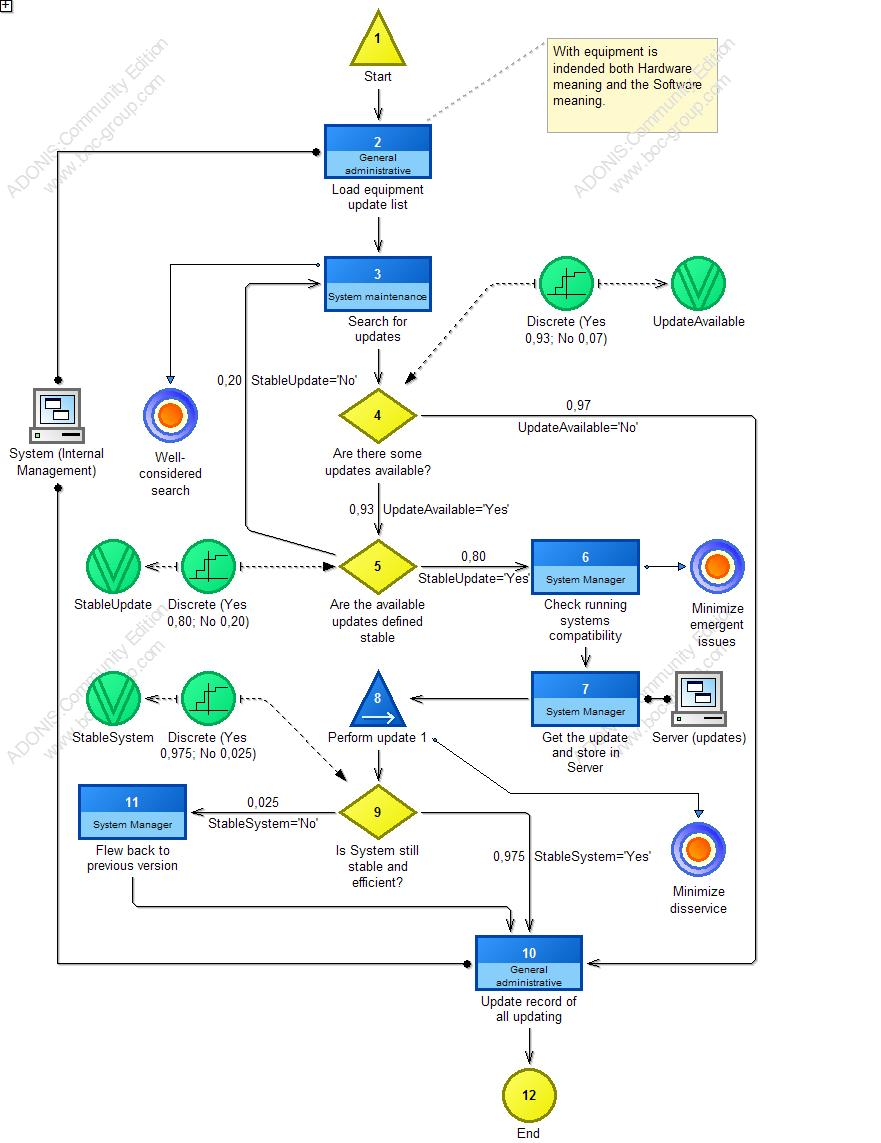
\includegraphics[scale=0.50]{assign2/adonis/imgs/updating.jpg}
\caption{AllSpark Updating Management.}
\label{2img:updating}
\end{centering}
\end{figure}


\subsubsection{Path Analysis}
According to the results of path analysis, an update is expected to succeed with the probability of 73,70\% as foreseen. The whole process is quite cheaper and the time is considered with nothing going badly. The following report returns the complete information about it.

\begin{alltt}
Probability:   73,7000\%
Execution time:  00:000:01:21:00
Waiting time:  00:000:00:02:00
Resting time:  00:000:00:12:00
Transport time:  00:000:00:10:00
Cycle time:  00:000:01:45:00
Costs:  1,980000

Updating Management 0.3 (Business process model)
========================================
Process start: Start
Activity: Load equipment update list
Activity: Search for updates
Decision: Are there some updates available? --> UpdateAvailable='Yes'
Decision: Are the available updates defined stable --> StableUpdate='Yes'
Activity: Check running systems compatibility
Activity: Get the update and store in Server
Subprocess: Perform update
Decision: Is System still stable and efficient? --> StableSystem='Yes'
Activity: Update record of all updating
End: End

Updating Management 0.3 (Business process model) --> Perform update 1 (Business process model)
========================================
Process start: Start
Activity: Perform update
End: End
\end{alltt}


\subsubsection{Capacity Analysis}
The capacity analysis for this process shows the interesting activites' report which are strongly dependent by the System Manager which is represented by either Sysadmin or Area Manager distinguishing the cases in which he is the real responsible of the entire AllSpark's system structure.

\begin{landscape}
\begin{table}
\centering
{\tiny
\begin{tabular}{|l|l|l|l|l|l|l|}
Business process&Activity&Performer&Number&Execution time&Cycle time&Costs\\
\hline
Updating Management 0.3&&&&00:000:01:23:33&00:000:01:48:07&5,966800\\
\hline
&Load equipment update list &&1,000000&00:000:00:01:00&&0,200000\\
\hline
&&Secretary &1,000000&00:000:00:01:00&&0,200000\\
\hline
&Update record of all updating &&1,000000&00:000:00:15:00&&0,900000\\
\hline
&&Secretary &1,000000&00:000:00:15:00&&0,900000\\
\hline
&Search for updates &&1,240000&00:000:00:24:48&&0,248000\\
\hline
&&Sysadmin &1,240000&00:000:00:24:48&&0,248000\\
\hline
&Check running systems compatibility &&0,910000&00:000:00:09:06&&0,273000\\
\hline
&&Area Manager &0,910000&00:000:00:09:06&&0,273000\\
\hline
&Flew back to previous version &&0,020000&00:000:00:01:48&&4,000000\\
\hline
&&Area Manager &0,020000&00:000:00:01:48&&4,000000\\
\hline
&Get the update and store in Server &&0,910000&00:000:00:13:39&&0,273000\\
\hline
&&Area Manager &0,910000&00:000:00:13:39&&0,273000\\
\hline
&Perform update &&0,910000&00:000:00:18:12&&0,072800\\
\hline
&&Sysadmin &0,910000&00:000:00:18:12&&0,072800\\
\hline
Total&&&&00:000:01:23:33&&5,966800
\end{tabular}
}
\caption{Capacity analysis for Updating Management.}
\end{table}
\end{landscape}
%

%

\subsection{Security checking}
The ``Security checking'' business process scope is to achieve the best protection through prevention against introuders, external penetration attempts, system's robustness and security, reliability with high load application and stability. To performing all the test, sometime is necessary to require a professional\footnote{In particular penetration test are aimed by AllSpark to certificate its quality.} that has experience in this kind of application and, over all, that is costantly up to date with respect to the always new method to trick the barriers.

Since the test concern both implemented product and the acquired product, the main responsible of all the operation is located on the Project management role which sorround all the aspect of the Company's system. The testing functionalities are followed also by some elements of ``Research \& Development'' organizational unit, represented in figure \ref{2img:working}, in order to furnish detailed parameters and to acquire testing metodologies.

\begin{figure}[ht!]
\begin{centering}
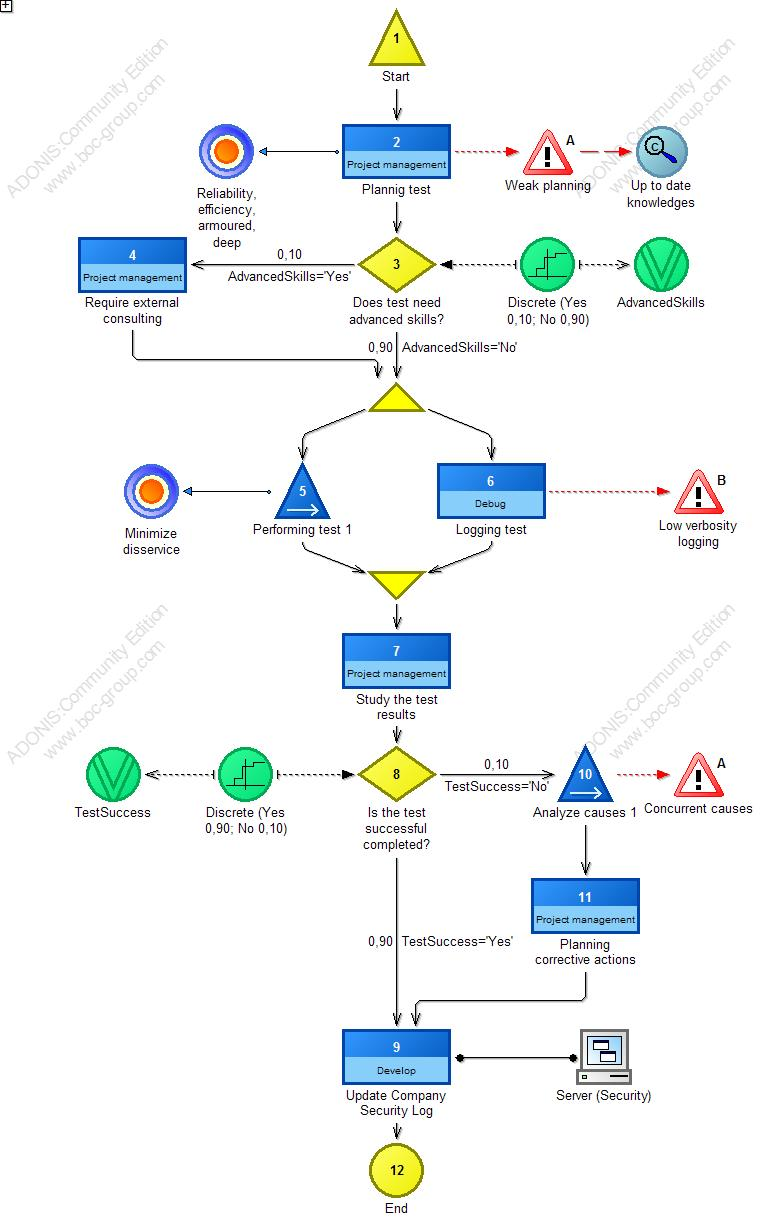
\includegraphics[scale=0.50]{assign2/adonis/imgs/security.jpg}
\caption{AllSpark Security checking.}
\label{2img:security}
\end{centering}
\end{figure}


\subsubsection{Path Analysis}
A path leads with the 80,20\% of probability above the all others resulting by the path analysis. The timing is quite interesting since in about two hours is possible to indicate the characteristics of the Systems. This time excludes eventually a deep penetration test which requires day of work in order to acquire sensitive information to use against the AllSpark.

\begin{alltt}
Probability:   80,2000\%
Execution time:  00:000:02:05:00
Waiting time:  00:000:00:03:00
Resting time:  00:000:00:00:00
Transport time:  00:000:00:05:00
Cycle time:  00:000:02:08:00
Costs:  2,510000

Security Checking 0.1 (Business process model)
========================================
Process start: Start
Activity: Plannig test
Decision: Does test need advanced skills? --> AdvancedSkills='No'
Parallelity: Parallelity-21893
    *
    Activity: Logging test
    *
    Subprocess: Performing test
Merging: Merging-21898
Activity: Study the test results
Decision: Is the test successful completed? --> TestSuccess='Yes'
Activity: Update Company Security Log
End: End

Security Checking 0.1 (Business process model) --> Performing test 1 (Business process model)
========================================
Process start: Start
Activity: Performing test
End: End
\end{alltt}


\subsubsection{Capacity Analysis}
The capacity analysis of this process shows the interesting variation of Execution time from the Cycle time. This element underline the great difference in the concept of real execution versus the concept of the factors that may involve in a determined task as in this case.

\begin{landscape}
\begin{table}
\centering
{\tiny
\begin{tabular}{|l|l|l|l|l|l|l|}
Business process&Activity&Performer&Number&Execution time&Cycle time&Costs\\
\hline
Security Checking 0.1&&&&00:000:02:14:24&00:000:03:24:49&8,014000\\
\hline
&Plannig test &&1,000000&00:000:00:20:00&&1,000000\\
\hline
&&Analyst &1,000000&00:000:00:20:00&&1,000000\\
\hline
&Require external consulting &&0,108000&00:000:00:01:05&&5,400000\\
\hline
&&Analyst &0,108000&00:000:00:01:05&&5,400000\\
\hline
&Logging test &&1,000000&00:000:00:05:00&&0,010000\\
\hline
&&Programmer &1,000000&00:000:00:05:00&&0,010000\\
\hline
&Study the test results &&1,000000&00:000:00:30:00&&0,500000\\
\hline
&&Analyst &1,000000&00:000:00:30:00&&0,500000\\
\hline
&Planning corrective actions &&0,104000&00:000:00:02:05&&0,052000\\
\hline
&&Analyst &0,104000&00:000:00:02:05&&0,052000\\
\hline
&Update Company Security Log &&1,000000&00:000:00:10:00&&0,000000\\
\hline
&&Programmer &1,000000&00:000:00:10:00&&0,000000\\
\hline
&Performing test &&1,000000&00:000:01:00:00&&1,000000\\
\hline
&&Area Manager &1,000000&00:000:01:00:00&&1,000000\\
\hline
&Performing test &&0,104000&00:000:00:06:14&&0,052000\\
\hline
&&Area Manager &0,104000&00:000:00:06:14&&0,052000\\
\hline
Total&&&&00:000:02:14:24&&8,014000
\end{tabular}
}
\caption{Capacity analysis for Security checking.}
\end{table}
\end{landscape}
%

%

\subsection{Supply Management}
The ``Supply Management'' business process models the procedure to achieve an internal store filled with the most required spares, indended also in the soft meaning such as original copies of software products. The major aim of this task is to manage the status of the basic element costitutional the Systems forseen the future needing.

All the activities have as performer the Secretary with different roles, but the entire process is supervised by the CEO who has to approve the business transaction with the supplier.

\begin{figure}[ht!]
\begin{centering}
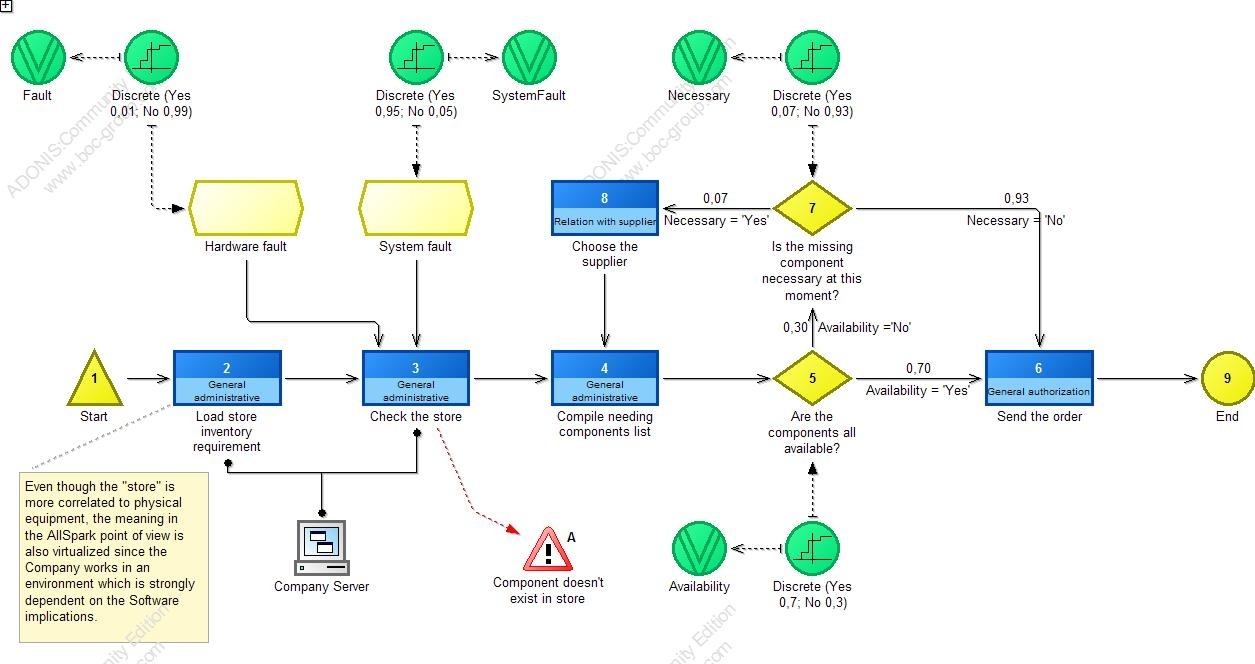
\includegraphics[scale=0.50, angle=90]{assign2/adonis/imgs/supply_man.jpg}
\caption{AllSpark Supply Management.}
\label{2img:supply_man}
\end{centering}
\end{figure}


\subsubsection{Path Analysis}
The analysis of possible path in this process shows five distinct elements, two of them with relevant probability. The most significative is the one with the 72,10\% of probability to happen and shows the favorite and expected actions with the needed components immediately available.

\begin{alltt}
Probability:   72,1000%
Execution time:  00:000:00:25:40
Waiting time:  00:000:00:00:50
Resting time:  00:000:00:00:20
Transport time:  00:000:00:00:00
Cycle time:  00:000:00:26:50
Costs:  2,000000

Supply Management 0.3 (Business process model)
========================================
Process start: Start
Activity: Load store inventory requirement
Activity: Check the store
Activity: Compile needing components list
Decision: Are the components all available? --> Availability = 'Yes'
Activity: Send the order
End: End
\end{alltt}


\subsubsection{Capacity Analysis}
This process is pretty simple and the variation from expected timing and costs are really small and the capacity analysis is according to the forseen result. By the way this process doesn't take account of the actual ending time that is the moment the order arrives at the AllSpark, but this is very diffult to model since is high dependent on the elements which the Company is looking for and an average would being be quite irrealistic.

\begin{landscape}
\begin{table}
\centering
{\tiny
\begin{tabular}{|l|l|l|l|l|l|l|}
Business process&Activity&Performer&Number&Execution time&Cycle time&Costs\\
\hline
Supply Management 0.3&&&&00:000:00:26:03&00:000:00:27:14&2,030000\\
\hline
&Choose the supplier &&0,015000&00:000:00:00:09&&0,030000\\
\hline
&&Secretary &0,015000&00:000:00:00:09&&0,030000\\
\hline
&Send the order &&1,000000&00:000:00:00:10&&0,000000\\
\hline
&&CEO &1,000000&00:000:00:00:10&&0,000000\\
\hline
&Compile needing components list &&1,015000&00:000:00:15:14&&0,000000\\
\hline
&&Secretary &1,015000&00:000:00:15:14&&0,000000\\
\hline
&Check the store &&1,000000&00:000:00:10:00&&2,000000\\
\hline
&&Secretary &1,000000&00:000:00:10:00&&2,000000\\
\hline
&Load store inventory requirement &&1,000000&00:000:00:00:30&&0,000000\\
\hline
&&Secretary &1,000000&00:000:00:00:30&&0,000000\\
\hline
Total&&&&00:000:00:26:03&&2,030000
\end{tabular}
}
\caption{Capacity analysis for Supply Management.}
\end{table}
\end{landscape}
%

%

\subsection{Human Resource Management}
The Human Resource Management business process aim to lead the main resource of the Company, that is the personnel. A good management of this resource facilitates the internal relations, improves the Company renown and image, reduce the stress factor and improve the productivity. There are several activities illustrates in figure \ref{2img:human_resources}, that combine to achieve the target. In first analysis is possibile to see that a lot of human relations are considered in this model, while the others more standard are relegated to subprocesses not shown here. The motivation is the peculiar orientation to the monitoring of variable factor that cannot be defined apriori.

A significantly number of activities are supervised by the Project Manager that is the role which best fit with the topic of the process since it is across several kind of competences and its culture is better flexible to the themes proposed, even though an official professional figure may be important here.

\begin{figure}[ht!]
\begin{centering}
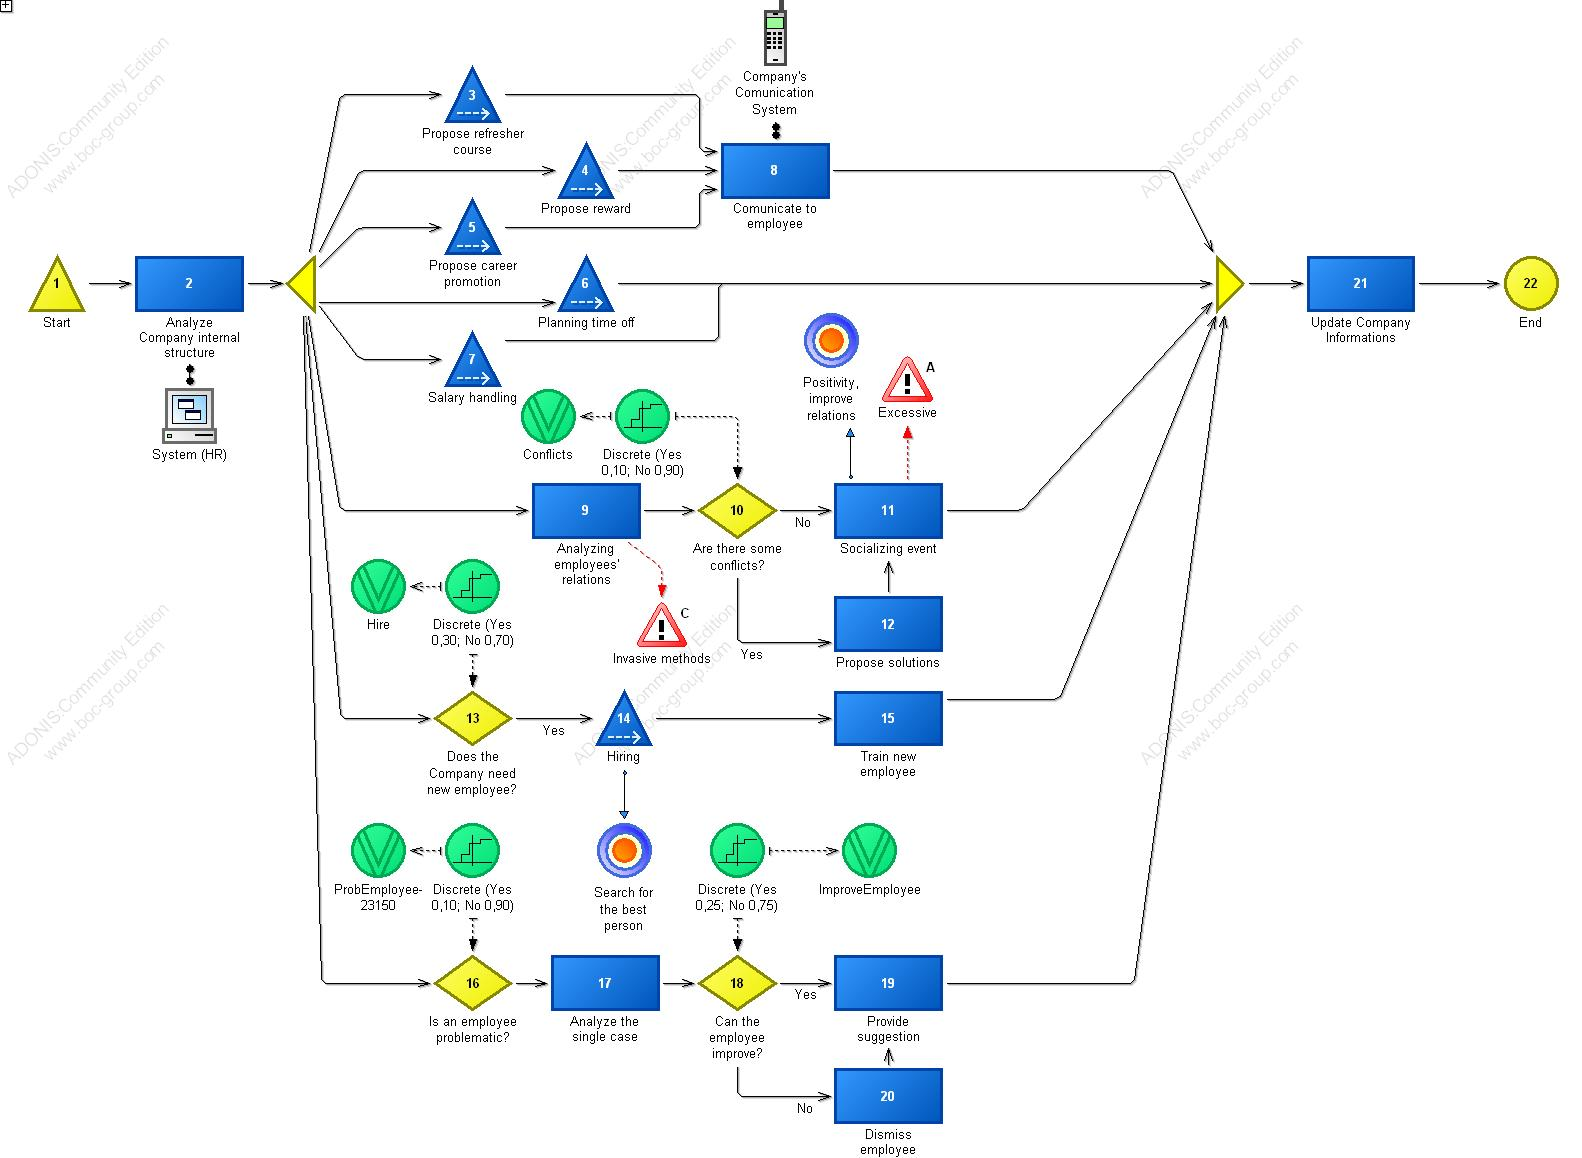
\includegraphics[scale=0.35, angle=90]{assign2/adonis/imgs/human_resources.jpg}
\caption{AllSpark Human Resources Management.}
\label{2img:human_resources}
\end{centering}
\end{figure}


\subsubsection{Path Analysis}
The path analysis results ten different paths, but only two of them are significative and are reported in the following table. Particular interesting the two paths shown differs significatively both in times and the costs even though this one is similar to the other. The two paths are completely shown straight forward the table.

The main difference is the hiring activity that requires a lot of resources to perform the task since a new element should be trained for, specially if is a young man with few experience.

Since all the activities are human's measured, is quite normal to have these results.

\begin{table}
\centering
\begin{tabular}{|l|l|l|l|l|}
Path&Probability&Execution time&Cycle time&Costs\\
\hline
1&0,5850&00:000:08:40:00&00:000:07:36:00&2060,65\\
\hline
2&0,2430&00:016:03:40:00&00:000:21:25:00&3075,65
\end{tabular}
\end{table}

\begin{alltt}
Probability:   58,5000%
Execution time:  00:000:08:40:00
Waiting time:  00:000:00:28:00
Resting time:  00:000:01:15:00
Transport time:  00:000:02:03:00
Cycle time:  00:000:07:36:00
Costs:  2060,650000

Human Resource Management 0.1 (Business process model)
========================================
Process start: Start
Activity: Analyze Company internal structure
Parallelity: Parallelity-23097
    *
    Activity: Analyzing employees' relations
    Decision: Are there some conflicts? --> Conflicts='No'
    Activity: Socializing event
    *
    Decision: Does the Company need new employee? --> Hire = 'No'
    *
    Decision: Is an employee problematic? --> Problematic='No'
    *
    Subprocess: Salary handling
    *
    Subprocess: Planning time off
    *
    Subprocess: Propose refresher course
    Activity: Comunicate to employee
    *
    Subprocess: Propose career promotion
    Activity: Comunicate to employee
    *
    Subprocess: Propose reward
    Activity: Comunicate to employee
Merging: Merging-23184
Activity: Update Company Informations
End: End

Human Resource Management 0.1 (Business process model) --> Salary handling 1 (Business process model)
========================================
Process start: Start
Activity: Salary handling
End: End

Human Resource Management 0.1 (Business process model) --> Planning time off 1 (Business process model)
========================================
Process start: Start
Activity: Planning time off
End: End

Human Resource Management 0.1 (Business process model) --> Propose refresher course 1 (Business process model)
========================================
Process start: Start
Activity: Refresh course
End: End

Human Resource Management 0.1 (Business process model) --> Propose career promotion 1 (Business process model)
========================================
Process start: Start
Activity: Career promotion
End: End

Human Resource Management 0.1 (Business process model) --> Propose reward 1 (Business process model)
========================================
Process start: Start
Activity: Reward
End: End
\end{alltt}

\begin{alltt}
Probability:   24,3000%
Execution time:  00:016:03:40:00
Waiting time:  00:002:00:38:00
Resting time:  00:003:02:15:00
Transport time:  00:001:02:03:00
Cycle time:  00:021:06:25:00
Costs:  3075,650000

Human Resource Management 0.1 (Business process model)
========================================
Process start: Start
Activity: Analyze Company internal structure
Parallelity: Parallelity-23097
    *
    Activity: Analyzing employees' relations
    Decision: Are there some conflicts? --> Conflicts='No'
    Activity: Socializing event
    *
    Decision: Does the Company need new employee? --> Hire='Yes'
    Subprocess: Hiring
    Activity: Train new employee
    *
    Decision: Is an employee problematic? --> Problematic='No'
    *
    Subprocess: Salary handling
    *
    Subprocess: Planning time off
    *
    Subprocess: Propose refresher course
    Activity: Comunicate to employee
    *
    Subprocess: Propose career promotion
    Activity: Comunicate to employee
    *
    Subprocess: Propose reward
    Activity: Comunicate to employee
Merging: Merging-23184
Activity: Update Company Informations
End: End

Human Resource Management 0.1 (Business process model) --> Salary handling 1 (Business process model)
========================================
Process start: Start
Activity: Salary handling
End: End

Human Resource Management 0.1 (Business process model) --> Planning time off 1 (Business process model)
========================================
Process start: Start
Activity: Planning time off
End: End

Human Resource Management 0.1 (Business process model) --> Propose refresher course 1 (Business process model)
========================================
Process start: Start
Activity: Refresh course
End: End

Human Resource Management 0.1 (Business process model) --> Propose career promotion 1 (Business process model)
========================================
Process start: Start
Activity: Career promotion
End: End

Human Resource Management 0.1 (Business process model) --> Propose reward 1 (Business process model)
========================================
Process start: Start
Activity: Reward
End: End

Human Resource Management 0.1 (Business process model) --> Hiring 1 (Business process model)
========================================
Process start: Start
Activity: Hiring
End: End
\end{alltt}


\subsubsection{Capacity Analysis}
In capacity analysis figure a sensible difference between the execution time and the cycle time consisting in about two days. A great contribute for the execution time is given with the hiring functions which is executed for a total of 0,30 times, but contribute significatively on the execution time. The costs are interesting particular the reward that is fixed as the attribute number indicates. Also socializing event is predetermined and this reflect the interesting of AllSpark to improve the internal relations.


\begin{landscape}
\begin{table}
\centering
{\tiny
\begin{tabular}{|l|l|l|l|l|l|l|}
Business process&Activity&Performer&Number&Execution time&Cycle time&Costs\\
\hline
Human Resource Management 0.1&&&&00:005:06:06:13&00:007:01:17:21&2372,965800\\
\hline
&Analyze Company internal structure &&1,000000&00:000:00:00:00&&0,000000\\
\hline
&&Secretary &1,000000&00:000:00:00:00&&0,000000\\
\hline
&Analyzing employees' relations &&1,000000&00:000:00:30:00&&0,300000\\
\hline
&&Area Manager &1,000000&00:000:00:30:00&&0,300000\\
\hline
&Propose solutions &&0,097000&00:000:00:05:49&&1,940000\\
\hline
&&Area Manager &0,097000&00:000:00:05:49&&1,940000\\
\hline
&Analyze the single case &&0,077000&00:000:00:02:19&&0,770000\\
\hline
&&Area Manager &0,077000&00:000:00:02:19&&0,770000\\
\hline
&Provide suggestion &&0,077000&00:000:00:00:46&&0,030800\\
\hline
&&Area Manager &0,077000&00:000:00:00:46&&0,030800\\
\hline
&Dismiss employee &&0,054000&00:000:00:00:49&&0,000000\\
\hline
&&CEO &0,054000&00:000:00:00:49&&0,000000\\
\hline
&Socializing event &&1,000000&00:000:01:00:00&&200,000000\\
\hline
&&CEO &1,000000&00:000:01:00:00&&200,000000\\
\hline
&Update Company Informations &&1,000000&00:000:00:10:00&&0,200000\\
\hline
&&Secretary &1,000000&00:000:00:10:00&&0,200000\\
\hline
&Comunicate to employee &&3,000000&00:000:00:30:00&&0,150000\\
\hline
&&Secretary &3,000000&00:000:00:30:00&&0,150000\\
\hline
&Train new employee &&0,305000&00:000:01:31:30&&4,575000\\
\hline
&&Area Manager &0,305000&00:000:01:31:30&&4,575000\\
\hline
&Refresh course &&1,000000&00:000:04:00:00&&200,000000\\
\hline
&&Area Manager &1,000000&00:000:04:00:00&&200,000000\\
\hline
&Reward &&1,000000&00:000:00:30:00&&1500,000000\\
\hline
&&CEO &1,000000&00:000:00:30:00&&1500,000000\\
\hline
&Career promotion &&1,000000&00:000:00:30:00&&100,000000\\
\hline
&&CEO &1,000000&00:000:00:30:00&&100,000000\\
\hline
&Planning time off &&1,000000&00:000:01:00:00&&10,000000\\
\hline
&&Area Manager &1,000000&00:000:01:00:00&&10,000000\\
\hline
&Salary handling &&1,000000&00:000:00:30:00&&50,000000\\
\hline
&&CEO &1,000000&00:000:00:30:00&&50,000000\\
\hline
&Hiring &&0,305000&00:004:05:45:00&&305,000000\\
\hline
&&CEO &0,305000&00:004:05:45:00&&305,000000\\
\hline
Total&&&&00:005:06:06:13&&2372,965800
\end{tabular}
}
\caption{Capacity analysis for Supply Management.}
\end{table}
\end{landscape}
%

%

\subsection{Updating Management}
This Updating Management business process is derived by the macro business process ``Systems Management'' that provides, as the name suggests, the service of ``up to date'' systems meaning softwares, both products and tools, and hardwares in order to minimize the presence of bugs, improve the efficiency and acquire new features.

The main responsible of this business process is the System Manager who has the very important role of manage all the tasks reducing the possible side effects. For certain task the System Manager is not required to be responsible since are not warning activities. The whole process is shown in figure \ref{2img:updating}.

\begin{figure}[ht!]
\begin{centering}
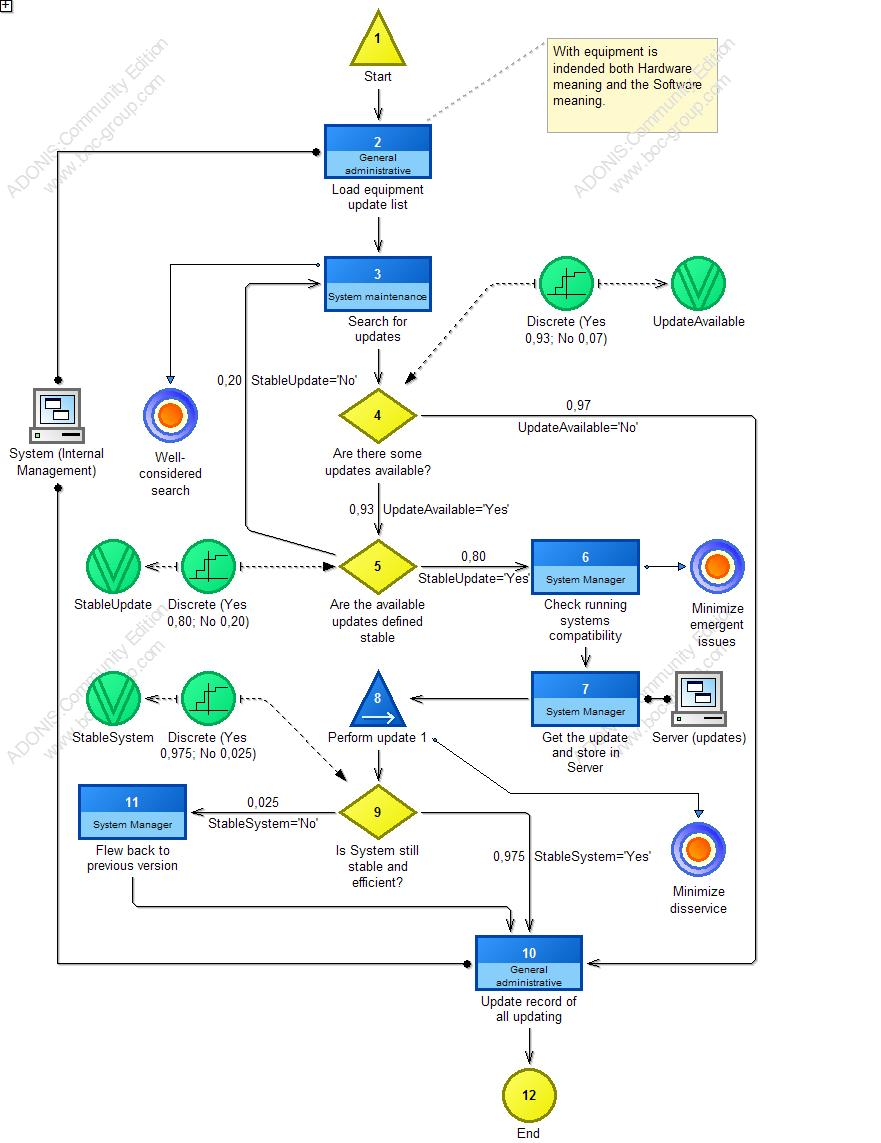
\includegraphics[scale=0.50]{assign2/adonis/imgs/updating.jpg}
\caption{AllSpark Updating Management.}
\label{2img:updating}
\end{centering}
\end{figure}


\subsubsection{Path Analysis}
According to the results of path analysis, an update is expected to succeed with the probability of 73,70\% as foreseen. The whole process is quite cheaper and the time is considered with nothing going badly. The following report returns the complete information about it.

\begin{alltt}
Probability:   73,7000\%
Execution time:  00:000:01:21:00
Waiting time:  00:000:00:02:00
Resting time:  00:000:00:12:00
Transport time:  00:000:00:10:00
Cycle time:  00:000:01:45:00
Costs:  1,980000

Updating Management 0.3 (Business process model)
========================================
Process start: Start
Activity: Load equipment update list
Activity: Search for updates
Decision: Are there some updates available? --> UpdateAvailable='Yes'
Decision: Are the available updates defined stable --> StableUpdate='Yes'
Activity: Check running systems compatibility
Activity: Get the update and store in Server
Subprocess: Perform update
Decision: Is System still stable and efficient? --> StableSystem='Yes'
Activity: Update record of all updating
End: End

Updating Management 0.3 (Business process model) --> Perform update 1 (Business process model)
========================================
Process start: Start
Activity: Perform update
End: End
\end{alltt}


\subsubsection{Capacity Analysis}
The capacity analysis for this process shows the interesting activites' report which are strongly dependent by the System Manager which is represented by either Sysadmin or Area Manager distinguishing the cases in which he is the real responsible of the entire AllSpark's system structure.

\begin{landscape}
\begin{table}
\centering
{\tiny
\begin{tabular}{|l|l|l|l|l|l|l|}
Business process&Activity&Performer&Number&Execution time&Cycle time&Costs\\
\hline
Updating Management 0.3&&&&00:000:01:23:33&00:000:01:48:07&5,966800\\
\hline
&Load equipment update list &&1,000000&00:000:00:01:00&&0,200000\\
\hline
&&Secretary &1,000000&00:000:00:01:00&&0,200000\\
\hline
&Update record of all updating &&1,000000&00:000:00:15:00&&0,900000\\
\hline
&&Secretary &1,000000&00:000:00:15:00&&0,900000\\
\hline
&Search for updates &&1,240000&00:000:00:24:48&&0,248000\\
\hline
&&Sysadmin &1,240000&00:000:00:24:48&&0,248000\\
\hline
&Check running systems compatibility &&0,910000&00:000:00:09:06&&0,273000\\
\hline
&&Area Manager &0,910000&00:000:00:09:06&&0,273000\\
\hline
&Flew back to previous version &&0,020000&00:000:00:01:48&&4,000000\\
\hline
&&Area Manager &0,020000&00:000:00:01:48&&4,000000\\
\hline
&Get the update and store in Server &&0,910000&00:000:00:13:39&&0,273000\\
\hline
&&Area Manager &0,910000&00:000:00:13:39&&0,273000\\
\hline
&Perform update &&0,910000&00:000:00:18:12&&0,072800\\
\hline
&&Sysadmin &0,910000&00:000:00:18:12&&0,072800\\
\hline
Total&&&&00:000:01:23:33&&5,966800
\end{tabular}
}
\caption{Capacity analysis for Updating Management.}
\end{table}
\end{landscape}
%

%

\subsection{Documentation repository}
The ``Documentation repository'' is another business process that is not directly connected to productivity or to the Company's lifecycle, but is needed to clearify the products in order to give to client a professional description, but also to facilitate future works based upon it. Particulary the process aim to draw up both commeting information on the project's files and the separated official documentation (that is both the documentation project and the documentation of use).

The main responsible of the task is the Analyst that supervise all the main activities. Also important are the role of Developer (who may be also a sysadmin if the topic is inherent the Systems) and Secretary who direct works on the documentation's building.

\begin{figure}[ht!]
\begin{centering}
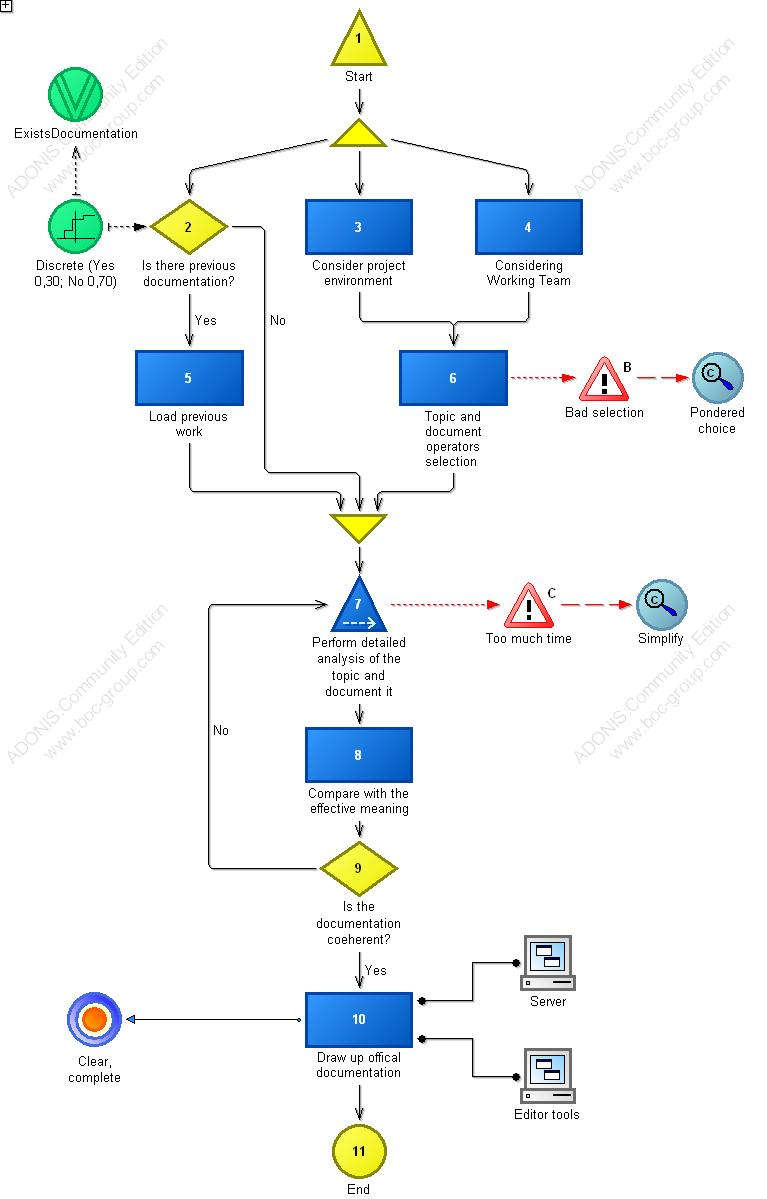
\includegraphics[scale=0.50]{assign2/adonis/imgs/documentation.jpg}
\caption{AllSpark Documentation repository.}
\label{2img:documentation}
\end{centering}
\end{figure}


\subsubsection{Path Analysis}
The path analysis return seven possible paths. Only two of them are interesting in terms of probability, but they are quite identical so only the most probability will be shown. The time is very low for a documentation and this is strange, but is important to underline that the process was modeled bearing that a project have at least a person, but may be different; this time is about the one person work and so the entire business process should be calibrate for each possible project which involve different people.

\begin{alltt}
Probability:   60,3000\%
Execution time:  00:000:03:20:00
Waiting time:  00:000:00:01:00
Resting time:  00:000:00:50:00
Transport time:  00:000:00:00:00
Cycle time:  00:000:03:16:00
Costs:  4,300000

Documentation repository 0.1 (Business process model)
========================================
Process start: Start
Parallelity: Parallelity-22082
    *
    Activity: Consider project environment
    Activity: Topic and document operators selection 
    *
    Activity: Considering Working Team
    Activity: Topic and document operators selection 
    *
    Decision: Is there previous documentation? --> ExistsDocumentation='No'
Merging: Merging-22112
Subprocess: Perform detailed analysis of the topic and document it
Activity: Compare with the effective meaning
Decision: Is the documentation coeherent? --> DocumentCoherency='Yes'
Activity: Draw up offical documentation
End: End

Documentation repository 0.1 (Business process model) --> Document 1 (Business process model)
========================================
Process start: Start
Activity: Documentation
End: End
\end{alltt}


\subsubsection{Capacity Analysis}
The capacity analysis of this process permits to observe the difference between execution time and cycle time which is possible thanking the parallelism which permits to reduce the global timing.

\begin{landscape}
\begin{table}
\centering
{\tiny
\begin{tabular}{|l|l|l|l|l|l|l|}
Business process&Activity&Performer&Number&Execution time&Cycle time&Costs\\
\hline
Documentation repository 0.1&&&&00:000:03:51:20&00:000:03:34:20&4,614100\\
\hline
&Load previous work &&0,283000&00:000:00:14:09&&0,084900\\
\hline
&&Secretary &0,283000&00:000:00:14:09&&0,084900\\
\hline
&Consider project environment &&1,000000&00:000:00:20:00&&0,400000\\
\hline
&&Analyst &1,000000&00:000:00:20:00&&0,400000\\
\hline
&Considering Working Team &&1,000000&00:000:00:20:00&&0,400000\\
\hline
&&Area Manager &1,000000&00:000:00:20:00&&0,400000\\
\hline
&Draw up offical documentation &&1,000000&00:000:00:30:00&&1,500000\\
\hline
&&Programmer &1,000000&00:000:00:30:00&&1,500000\\
\hline
&Topic and document operators selection  &&2,000000&00:000:00:40:00&&0,800000\\
\hline
&&Analyst &2,000000&00:000:00:40:00&&0,800000\\
\hline
&Compare with the effective meaning &&1,191000&00:000:00:23:49&&0,476400\\
\hline
&&Analyst &1,191000&00:000:00:23:49&&0,476400\\
\hline
&Documentation &&1,191000&00:000:01:23:22&&0,952800\\
\hline
&&Programmer &1,191000&00:000:01:23:22&&0,952800\\
\hline
Total&&&&00:000:03:51:20&&4,614100
\end{tabular}
}
\caption{Capacity analysis for Document repository.}
\end{table}
\end{landscape}
%

%
\section{Research \& development}
This department of AllSpark is involved in all the activities related to
improve and realize new products as research projects. This sector is
considered a relevant one in the organization business, in fact this sector
has the aim to bring innovation and distinguish our products among the
competitors.

An important feature of this area is the strong collaboration between
AllSpark and various foundation operating in the OpenSource community
environment.
These collaborations are based on active support of AllSpark during the
development of their project. The support AllSpark is offering id mainly
focused on patching and bugfixing, but can be expanded to founding or other
ways of collaboration.

\subsection{Search Sector}
The main aim of this process is to look for a research sector in which
instantiate a new r\&d project. Mainly is devolved to handle security
related sectors, due to the high risks and frequent changes always present
in this area.

The process involves an analysis of the newest studies on security issues
and menaces in IT systems, its results are useful for performing an
investigation about possible vulnerabilities in AllSparks products. Is
important to notice that other than check a single product is important to
consider the whole offer of AllSpark, looking for possible problems which
are not covered by the existing products but still in the scope of AllSpark
activity.

Image \ref{2img:sector} describes this process in its details.

\begin{figure}[!ht]
\begin{centering}
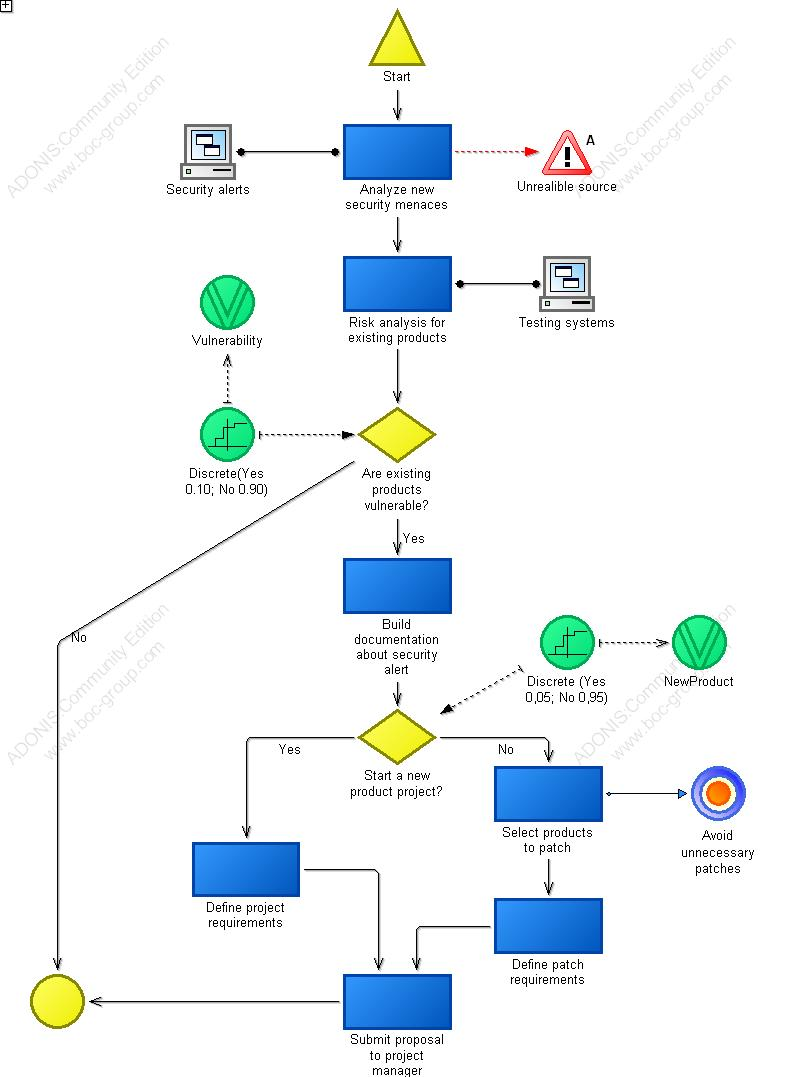
\includegraphics[scale=0.50]{assign2/adonis/imgs/sector.jpg}
\caption{Search sector AllSpark process}
\label{2img:sector}
\end{centering}
\end{figure}

\subsubsection{Path Analysis}
The result of the path analysis, shows that the most probable results is
that there are no such menaces which can trigger the starting of a new
research project.

This is a key point for reliability and marketing target for AllSpark's product and are aligned with the chosed directions.

\begin{table}[ht!]
\centering
\begin{tabular}{|l|l|l|l|l|}
\hline
Path&Probability&Execution time&Cycle time&Costs\\
\hline
1&0,899000&00:000:02:30:00&00:000:02:30:00&6,000000\\
\hline
2&0,092000&00:000:03:07:00&00:000:03:07:00&7,400000\\
\hline
3&0,009000&00:000:03:02:00&00:000:03:02:00&7,700000\\
\hline
\end{tabular}
\end{table}

\begin{alltt}
Probability:   89,9000%
Execution time:  00:000:02:30:00
Waiting time:  00:000:00:00:00
Resting time:  00:000:00:00:00
Transport time:  00:000:00:00:00
Cycle time:  00:000:02:30:00
Costs:  6,000000

Search sector 0.3 (Business process model)
========================================
Process start: Start
Activity: Analyze new security menaces
Activity: Risk analysis for existing products
Decision: Are existing products vulnerable? --> Vulnerability = 'No'
End: End
\end{alltt}

\subsubsection{Capacity Analysis}
Table \ref{2tab:sector} depicts the capacity analysis for the process of
searching a sector in which start a new research project.

Both Execution time and Cycle time agrees with the expected parameter forseen by the Company and so no improvement are needed.

\begin{landscape}
\centering
\begin{table}
{\tiny
\begin{tabular}{|l|l|l|l|l|l|l|}
Business process&Activity&Performer&Number&Execution time&Cycle
time&Costs\\
\hline
Search sector 0.3&&&&00:000:02:33:42&00:000:02:33:42&6,143200\\
\hline
&Analyze new security menaces &&1,000000&00:000:00:30:00&&1,000000\\
\hline
&&Area Manager &1,000000&00:000:00:30:00&&1,000000\\
\hline
&Risk analysis for existing products &&1,000000&00:000:02:00:00&&5,000000\\
\hline
&&Area Manager &1,000000&00:000:02:00:00&&5,000000\\
\hline
&Build documentation about security alert &&0,101000&00:000:00:02:01&&0,050500\\
\hline
&&Area Manager &0,101000&00:000:00:02:01&&0,050500\\
\hline
&Select products to patch &&0,095000&00:000:00:00:29&&0,047500\\
\hline
&&Programmer &0,049000&00:000:00:00:15&&0,024500\\
\hline
&&Analyst &0,046000&00:000:00:00:14&&0,023000\\
\hline
&Define project requirements &&0,006000&00:000:00:00:04&&0,006000\\
\hline
&&Area Manager &0,006000&00:000:00:00:04&&0,006000\\
\hline
&Define patch requirements &&0,095000&00:000:00:00:57&&0,019000\\
\hline
&&Area Manager &0,095000&00:000:00:00:57&&0,019000\\
\hline
&Submit proposal to project manager &&0,101000&00:000:00:00:12&&0,020200\\
\hline
&&Area Manager &0,101000&00:000:00:00:12&&0,020200\\
\hline
Total&&&&00:000:02:33:42&&6,143200\\
\hline
\end{tabular}
}
\caption{Capacity analysis for the process of selecting a sector for a new project} 
\label{2tab:sector}
\end{table}
\end{landscape}





\subsection{Search Updates}
In the IT environment trends and actual needs are often changing, is
therefore necessary to track these development in order to be prepared and
offer always updated products which can actually encounter costumer's
needs.

The aim of this process is to analyze the evolving market data and monitor
the trends in products usage. In this way AllSpark can retrieve a reliable
picture of the market trends.
The results of this analysis can be used to check whether there is the need
for developing a new product, or if is sufficient to add new features and
extensions to an existing one.

This process is depicted in image \ref{2img:search_upd}.

\begin{figure}[!ht]
\begin{centering}
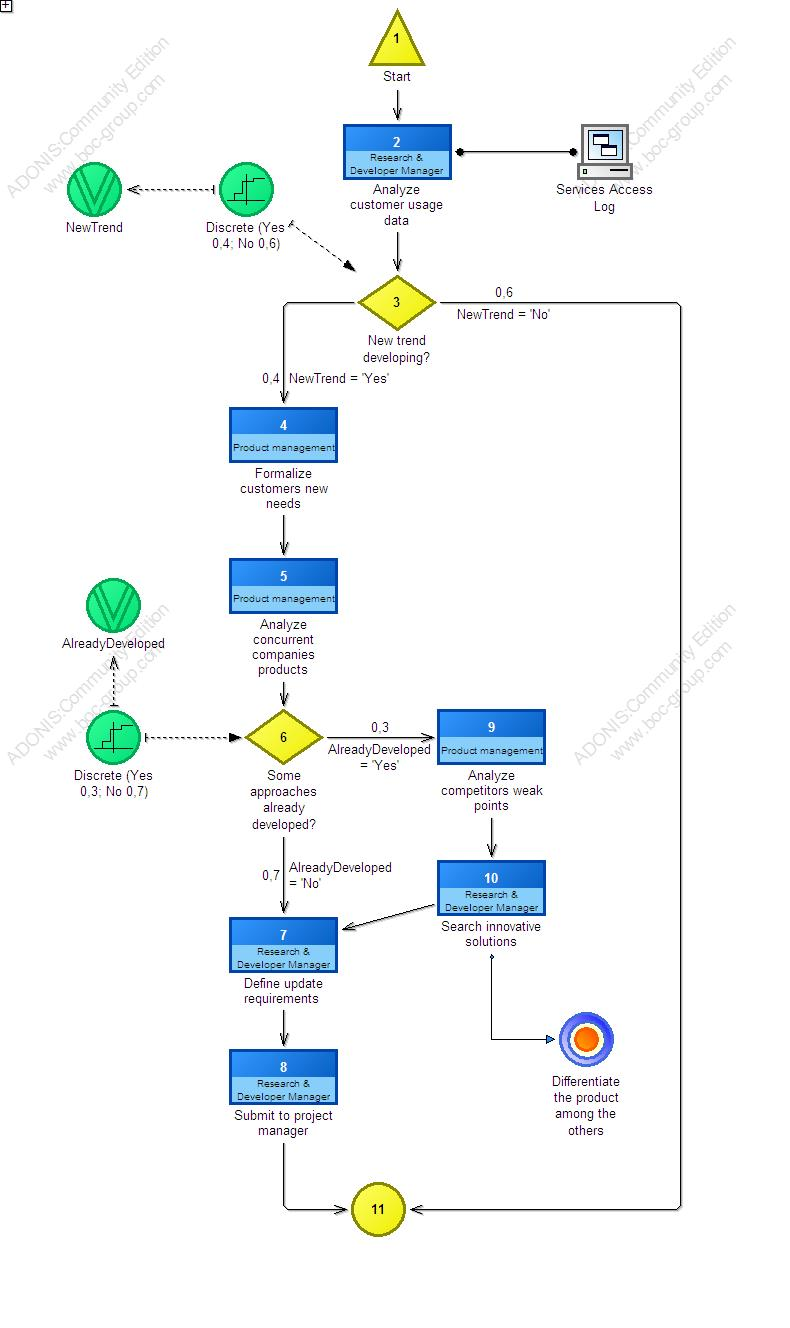
\includegraphics[scale=0.40]{assign2/adonis/imgs/search_upd.jpg}
\caption{Update searching process}
\label{2img:search_upd}
\end{centering}
\end{figure}

\subsubsection{Path Analysis}
The analysis of the possible paths shows that the evolution of the customer
trends, not always leads to the developing of new products.

The probability gathered by the analysis are in the same optics of the expectations even though a priori assumption of targeting should be done. The process manage actually the meaning of the AllSpark since each new update should be covered by a Working team that has to be redirected from other evolving project.

\begin{table}[ht!]
\centering
\begin{tabular}{|l|l|l|l|l|}
\hline
Path&Probability&Execution time&Cycle time&Costs\\
\hline
1&0,601000&00:000:00:10:00&00:000:00:10:00&2,000000\\
\hline
2&0,264000&00:000:01:52:00&00:000:01:52:00&67,200000\\
\hline
3&0,135000&00:000:03:37:00&00:000:03:37:00&217,200000\\
\hline
\end{tabular}
\end{table}

\begin{alltt}
Probability:   60,1000%
Execution time:  00:000:00:10:00
Waiting time:  00:000:00:00:00
Resting time:  00:000:00:00:00
Transport time:  00:000:00:00:00
Cycle time:  00:000:00:10:00
Costs:  2,000000

Search Updates 0.3 (Business process model)
========================================
Process start: Start
Activity: Analyze customer usage data
Decision: New trend developing? --> NewTrend = 'No'
End: End-44324
\end{alltt}

\subsubsection{Capacity Analysis}
Table \ref{2tab:updates} depicts the results of the capacity analysis of
this process where there aren't relevant conclusions to achieve, the results correctly fit the expectations.
\begin{landscape}
\centering
\begin{table}
{\tiny
\begin{tabular}{|l|l|l|l|l|l|l|}
Business process&Activity&Performer&Number&Execution time&Cycle
time&Costs\\
\hline
Search Updates 0.3&&&&00:000:01:03:53&00:000:01:03:53&45,812400\\
\hline
&Analyze customer usage data &&1,000000&00:000:00:10:00&&2,000000\\
\hline
&&Area Manager &1,000000&00:000:00:10:00&&2,000000\\
\hline
&Formalize customers new needs &&0,412000&00:000:00:08:14&&4,120000\\
\hline
&&Programmer &0,204000&00:000:00:04:05&&2,040000\\
\hline
&&Analyst &0,208000&00:000:00:04:10&&2,080000\\
\hline
&Analyze concurrent companies products &&0,412000&00:000:00:24:43&&20,600000\\
\hline
&&Programmer &0,206000&00:000:00:12:22&&10,300000\\
\hline
&&Analyst &0,206000&00:000:00:12:22&&10,300000\\
\hline
&Search innovative solutions &&0,113000&00:000:00:06:47&&11,300000\\
\hline
&&Area Manager &0,113000&00:000:00:06:47&&11,300000\\
\hline
&Define update requirements  &&0,412000&00:000:00:08:14&&2,060000\\
\hline
&&Area Manager &0,412000&00:000:00:08:14&&2,060000\\
\hline
&Analyze competitors weak points &&0,113000&00:000:00:05:05&&5,650000\\
\hline
&&Programmer &0,067000&00:000:00:03:01&&3,350000\\
\hline
&&Analyst &0,046000&00:000:00:02:04&&2,300000\\
\hline
&Submit to project manager &&0,412000&00:000:00:00:49&&0,082400\\
\hline
&&Area Manager &0,412000&00:000:00:00:49&&0,082400\\
\hline
Total&&&&00:000:01:03:53&&45,812400\\
\hline
\end{tabular}
}
\caption{Capacity analysis for the process of searching updates for a
product} 
\label{2tab:updates}
\end{table}
\end{landscape}



\subsection{Search bug}
This process describes how AllSpark handles with failures in its own
research project. In this process, in fact, developers are involved in
finding and fixing errors in existing projects.

In this process the main attention is focused on performing smart tests in
order to find and resolve the problems. One important thing is to notice
the difference between the two kinds of test which are going to be
performed.
In fact, after a first analysis of the code, is necessary to develop a
series of test cases which provides a wide coverage over the possible
different behaviour of the system. When the bug is located and a patch is
prepared, a sharper approach is needed, in order to test that particular
portion of the system. The process used in AllSpark to deal with bug
problems in research project is described in figure \ref{2img:search_bug}.

\begin{figure}[!ht]
\begin{centering}
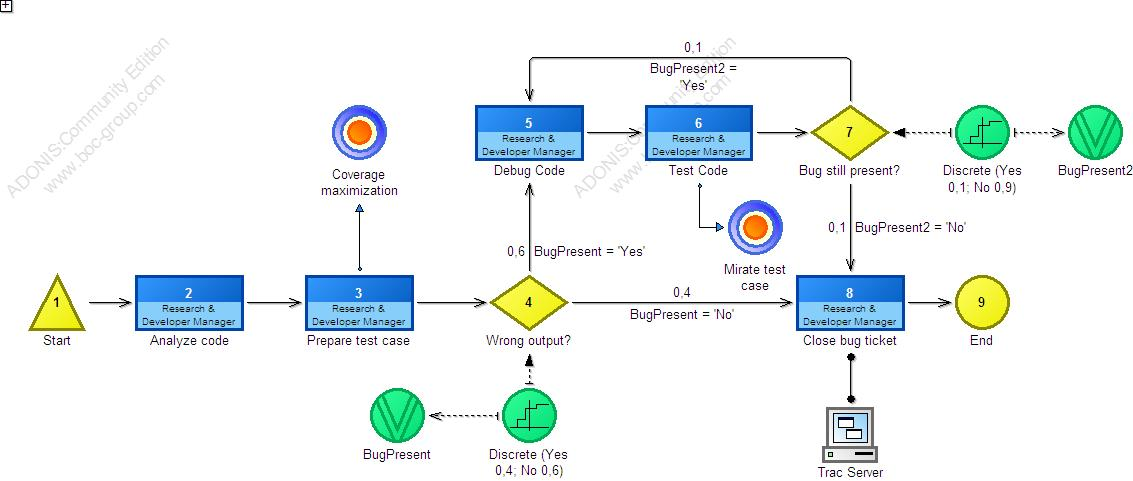
\includegraphics[scale=0.50, angle=90]{assign2/adonis/imgs/debug.jpg}
\caption{AllSparks debug process for Research project}
\label{2img:search_bug}
\end{centering}
\end{figure}

\subsubsection{Path Analysis}
The most probable path for this process determines the normal condition in
which no bugs are found in the analyzed application as expected by the AllSpark.

In case of bugs the execution time grows very quickly with the reducing of the probability. This is a forseen aspects that demostrate a correct representation of the real world environment.s


\begin{table}[ht!]
\centering
\begin{tabular}{|l|l|l|l|l|}
\hline
Path&Probability&Execution time&Cycle time&Costs\\
\hline
1&0,624000&00:000:01:15:00&00:000:01:15:00&11,400000\\
\hline
2&0,333000&00:001:01:45:00&00:001:01:45:00&221,400000\\
\hline
3&0,039000&00:002:02:15:00&00:002:02:15:00&431,400000\\
\hline
4&0,004000&00:003:02:45:00&00:003:02:45:00&641,400000\\
\hline
\end{tabular}
\end{table}

\begin{alltt}
Probability:   62,4000%
Execution time:  00:000:01:15:00
Waiting time:  00:000:00:00:00
Resting time:  00:000:00:00:00
Transport time:  00:000:00:00:00
Cycle time:  00:000:01:15:00
Costs:  11,400000

Search bug 0.3 (Business process model)
========================================
Process start: Start
Activity: Analyze code
Activity: Prepare test case
Decision: Wrong output? --> BugPresent = 'No'
Activity: Close bug ticket
End: End
\end{alltt}

\subsubsection{Capacity Analysis}
Table \ref{2tab:debug} is the result of the capacity analysis of this
process which is aligned with the expectations given.

\begin{landscape}
\centering
\begin{table}
{\tiny
\begin{tabular}{|l|l|l|l|l|l|l|}
Business process&Activity&Performer&Number&Execution time&Cycle
time&Costs\\
\hline
Search bug 0.3&&&&00:000:05:37:43&00:000:05:37:43&98,970000\\
\hline
&Analyze code &&1,000000&00:000:00:40:00&&1,000000\\
\hline
&&Area Manager &1,000000&00:000:00:40:00&&1,000000\\
\hline
&Prepare test case &&1,000000&00:000:00:30:00&&10,000000\\
\hline
&&Area Manager &1,000000&00:000:00:30:00&&10,000000\\
\hline
&Debug Code &&0,417000&00:000:04:10:12&&83,400000\\
\hline
&&Area Manager &0,417000&00:000:04:10:12&&83,400000\\
\hline
&Test Code &&0,417000&00:000:00:12:31&&4,170000\\
\hline
&&Area Manager &0,417000&00:000:00:12:31&&4,170000\\
\hline
&Close bug ticket &&1,000000&00:000:00:05:00&&0,400000\\
\hline
&&Area Manager &1,000000&00:000:00:05:00&&0,400000\\
\hline
Total&&&&00:000:05:37:43&&98,970000\\
\hline
\end{tabular}
}
\caption{Capacity analysis for the process of debugging a research project} 
\label{2tab:debug}
\end{table}
\end{landscape}



\subsection{Foundation Cooperation}
As said before, one of the aim of AllSpark is be engaged in an active
collaboration with the entities working in the OpenSource field. The
benefit of this collaboration is to be evaluated in an economic sense from
one side, and from a reputation point of view form the other.

For the foundations could be an opportunity to gain renown if AllSpark
products integrate their solutions. Apart from this the collaboration can
be based on financial founding or, as in the case of the research project,
on active collaboration on software developing.

This collaboration extends to bugfixing and patching the software, not to
strategic decisions on the direction of the development, this to preserve
the independence of the Foundation in its business.

The project of the patching activities for software not developed by
AllSpark, but by an OpenSource Foundation is described by figure
\ref{2img:found_coop}

\begin{figure}[!ht]
\begin{centering}
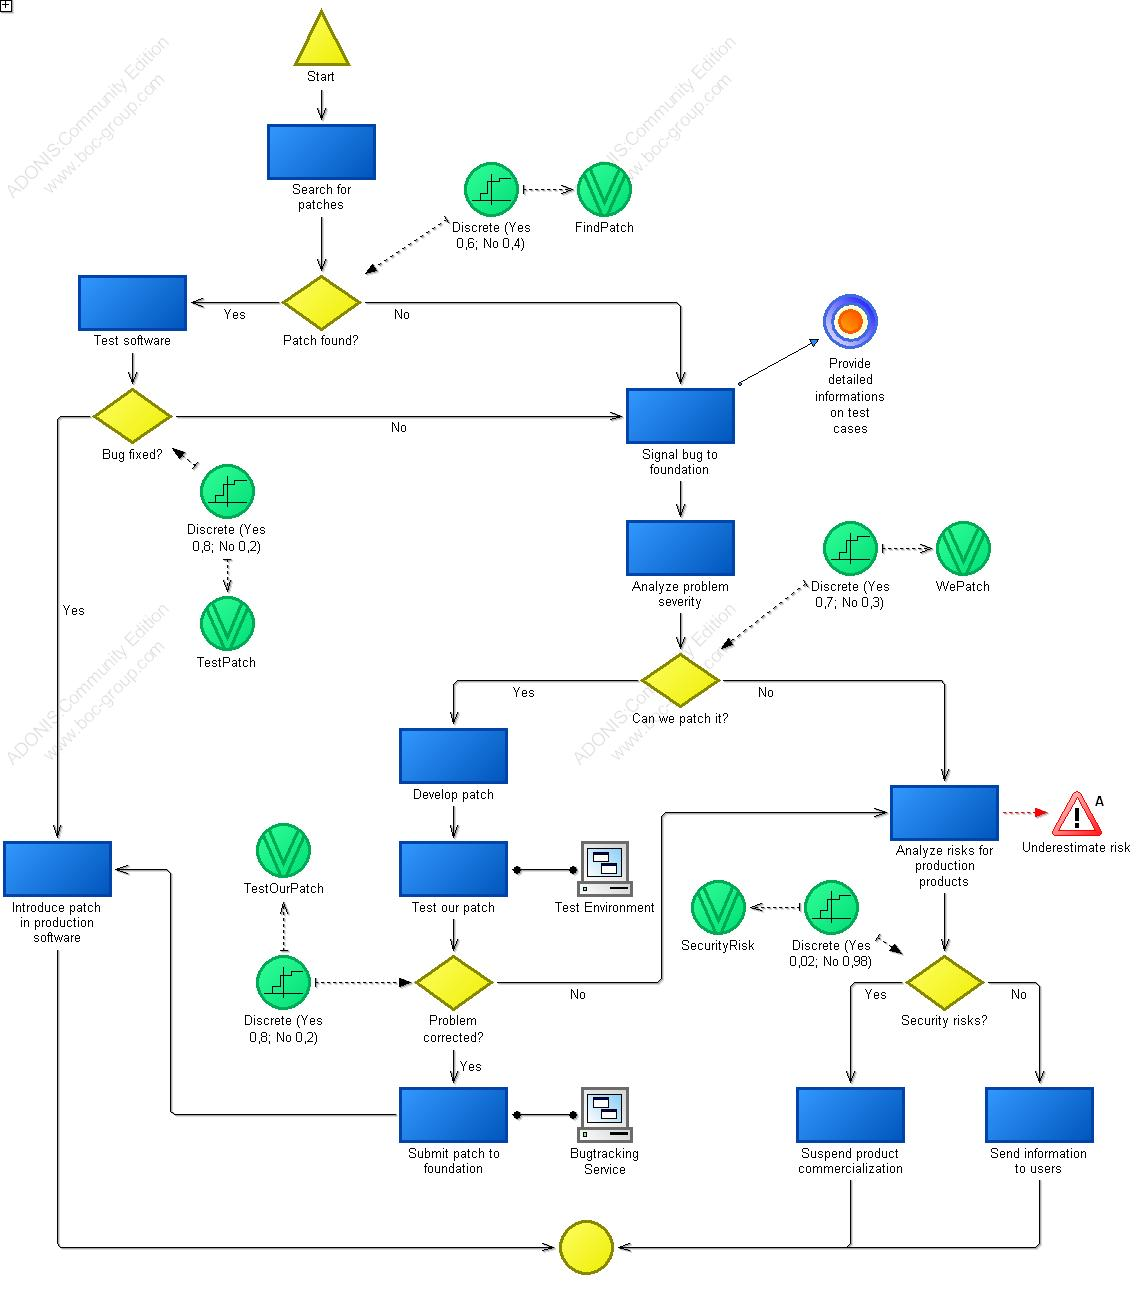
\includegraphics[scale=0.40]{assign2/adonis/imgs/coop.jpg}
\caption{Collaboration between AllSpark and OpenSource projects}
\label{2img:found_coop}
\end{centering}
\end{figure}

\subsubsection{Path Analysis}
The results of the path analysis of this process shows that the most
probable outcome of this process is that the Foundation has already
provided a working solution for the discovered problem.
The least probable paths are the ones in which neither AllSPark nor the
foundation are able to find a solution for a security related problem,
which lead to more important consequences.

\begin{table}[ht!]
\centering
\begin{tabular}{|l|l|l|l|l|}
\hline
Path&Probability&Execution&time&Costs\\
\hline
1&0,478000&00:000:04:00:00&00:000:04:00:00&151,000000\\
\hline
2&0,219000&00:010:03:55:00&00:010:03:55:00&662,000000\\
\hline
3&0,117000&00:000:01:53:00&00:000:01:53:00&31,000000\\
\hline
4&0,082000&00:010:05:25:00&00:010:05:25:00&762,000000\\
\hline
5&0,060000&00:010:01:58:00&00:010:01:58:00&631,000000\\
\hline
6&0,030000&00:000:03:23:00&00:000:03:23:00&131,000000\\
\hline
7&0,012000&00:010:03:28:00&00:010:03:28:00&731,000000\\
\hline
8&0,001000&00:000:04:13:00&00:000:04:13:00&211,000000\\
\hline
9&0,001000&00:010:04:18:00&00:010:04:18:00&811,000000\\
\hline
\end{tabular}
\end{table}

\begin{alltt}
Probability:   47,8000%
Execution time:  00:000:04:00:00
Waiting time:  00:000:00:00:00
Resting time:  00:000:00:00:00
Transport time:  00:000:00:00:00
Cycle time:  00:000:04:00:00
Costs:  151,000000

Foundations Coop 0.3 (Business process model)
========================================
Process start: Start
Activity: Search for patches
Decision: Patch found? --> FindPatch = 'Yes'
Activity: Test software
Decision: Bug fixed? --> TestPatch = 'Yes'
Activity: Introduce patch in production software
End: End-44485
\end{alltt}

\subsubsection{Capacity Analysis}
Table \ref{2tab:coop} shows how the work is divided among developers (for
the implementation part) and area manager for the analysis of product and
bug severity. 

The interesting combination of decision point results on the number of execution expected by the single activities, in particular ``Suspend product commercialization'' has a very low number of executions as the AllSpark aims to achieve.

\begin{landscape}
\centering
\begin{table}
{\tiny
\begin{tabular}{|l|l|l|l|l|l|l|}
Business process&Activity&Performer&Number&Execution time&Cycle
time&Costs\\
\hline
Foundations Coop 0.3&&&&00:004:02:40:34&00:004:02:40:34&341,990000\\
\hline
&Search for patches &&1,000000&00:000:00:30:00&&1,000000\\
\hline
&&Area Manager &1,000000&00:000:00:30:00&&1,000000\\
\hline
&Test software &&0,577000&00:000:00:51:56&&57,700000\\
\hline
&&Area Manager &0,577000&00:000:00:51:56&&57,700000\\
\hline
&Introduce patch in production software &&0,774000&00:000:01:32:53&&38,700000\\
\hline
&&Area Manager &0,774000&00:000:01:32:53&&38,700000\\
\hline
&Signal bug to foundation &&0,536000&00:000:00:05:22&&0,000000\\
\hline
&&Area Manager &0,536000&00:000:00:05:22&&0,000000\\
\hline
&Analyze problem severity &&0,536000&00:000:00:32:10&&5,360000\\
\hline
&&Area Manager &0,536000&00:000:00:32:10&&5,360000\\
\hline
&Develop patch &&0,390000&00:003:09:00:00&&195,000000\\
\hline
&&Area Manager &0,390000&00:003:09:00:00&&195,000000\\
\hline
&Test our patch &&0,390000&00:000:00:01:57&&39,000000\\
\hline
&&Area Manager &0,390000&00:000:00:01:57&&39,000000\\
\hline
&Submit patch to foundation &&0,310000&00:000:00:03:06&&0,310000\\
\hline
&&Area Manager &0,310000&00:000:00:03:06&&0,310000\\
\hline
&Analyze risks for production products &&0,226000&00:000:00:00:41&&0,000000\\
\hline
&&Programmer &0,115000&00:000:00:00:21&&0,000000\\
\hline
&&Analyst &0,111000&00:000:00:00:20&&0,000000\\
\hline
&Suspend product commercialization &&0,005000&00:000:00:00:18&&0,500000\\
\hline
&&Programmer &0,002000&00:000:00:00:07&&0,200000\\
\hline
&&Analyst &0,003000&00:000:00:00:11&&0,300000\\
\hline
&Send information to users &&0,221000&00:000:00:02:13&&4,420000\\
\hline
&&Area Manager &0,221000&00:000:00:02:13&&4,420000\\
\hline
Total&&&&00:004:02:40:34&&341,990000\\
\hline
\end{tabular}
}
\caption{Capacity analysis for the process of collaboration with an
OpenSource foundation} 
\label{2tab:coop}
\end{table}
\end{landscape}




\subsection{Commercialization}
This process manages the procedure executed to evaluate if a research
project is ready to be actually converted in a effective product.
Is important to notice that this decision depends on on the market data and
on the need of the customer.

It can be the case that a project is not ready to be commercialized, or,
instead, the project is ready but the market and the customers don't yet
need this new product, at this moment.

If this is the case, is necessary to delay the commercialization of the
product waiting for a moment in which it can be more appreciated.
This process is described in figure \ref{2img:commerce}

\begin{figure}[!ht]
\begin{centering}
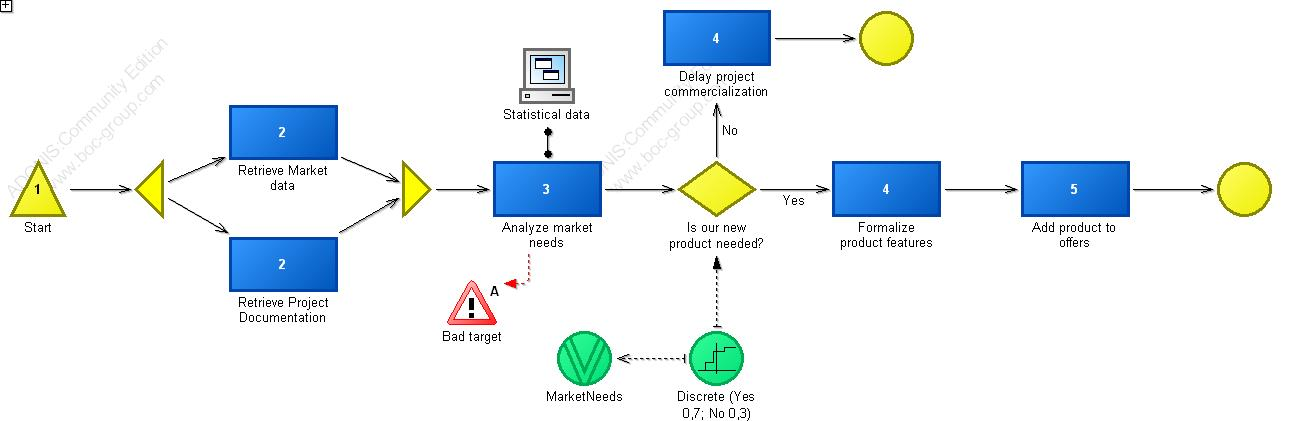
\includegraphics[scale=0.45,angle=90]{assign2/adonis/imgs/commercialize.jpg}
\caption{Commercialization of a research project}
\label{2img:commerce}
\end{centering}
\end{figure}

\subsubsection{Path Analysis}
The analysis of the possible paths shows that the most probable, with 71\%
pf probability, id that a project is accepted as a new product.
The other one, which leads to the delay of the commercialization of the
product, has a probability of 30\%.

\begin{table}[ht!]
\centering
\begin{tabular}{|l|l|l|l|l|}
Path&Probability&Execution&time&Costs\\
\hline
1&0,686000&00:000:00:46:00&00:000:00:43:00&110,400000\\
\hline
2&0,314000&00:000:00:28:00&00:000:00:25:00&5,400000\\
\hline
\end{tabular}
\end{table}


\begin{alltt}
Probability:   71,7000%
Execution time:  00:000:00:46:00
Waiting time:  00:000:00:00:00
Resting time:  00:000:00:00:00
Transport time:  00:000:00:00:00
Cycle time:  00:000:00:43:00
Costs:  110,400000

Commercializing 0.3 (Business process model)
========================================
Process start: Start
Parallelity: Parallelity-41066
    *
    Activity: Retrieve Project Documentation
    *
    Activity: Retrieve Market data
Merging: Merging-41072
Activity: Analyze market needs
Decision: Is our new product needed? --> MarketNeeds = 'Yes'
Activity: Formalize product features
Activity: Add product to offers
End: End-41103
\end{alltt}



\subsubsection{Capacity Analysis}
Table \ref{2tab:commerc} shows the capacity analysis for the roles involved in
the commercialization of a research project.
\begin{landscape}
\centering
\begin{table}
{\tiny
\begin{tabular}{|l|l|l|l|l|l|l|}
Business process&Activity&Performer&Number&Execution time&Cycle
time&Costs\\
\hline
Commercializing 0.3&&&&00:000:00:40:08&00:000:00:37:08&76,170000\\
\hline
&Retrieve Project Documentation &&1,000000&00:000:00:03:00&&0,200000\\
\hline
&&Area Manager &1,000000&00:000:00:03:00&&0,200000\\
\hline
&Retrieve Market data &&1,000000&00:000:00:03:00&&0,200000\\
\hline
&&Area Manager &1,000000&00:000:00:03:00&&0,200000\\
\hline
&Analyze market needs &&1,000000&00:000:00:20:00&&5,000000\\
\hline
&&Area Manager &1,000000&00:000:00:20:00&&5,000000\\
\hline
&Formalize product features &&0,674000&00:000:00:10:07&&3,370000\\
\hline
&&Area Manager &0,674000&00:000:00:10:07&&3,370000\\
\hline
&Add product to offers &&0,674000&00:000:00:03:22&&67,400000\\
\hline
&&Programmer &0,340000&00:000:00:01:42&&34,000000\\
\hline
&&Analyst &0,334000&00:000:00:01:40&&33,400000\\
\hline
&Delay project commercialization &&0,326000&00:000:00:00:39&&0,000000\\
\hline
&&Area Manager &0,326000&00:000:00:00:39&&0,000000\\
\hline
\end{tabular}
}
\caption{Capacity analysis for the process of commercialization of a
research project}
\label{2tab:commerc}
\end{table}
\end{landscape}




\section{Course Management}
Another important sector in which AllSpark is involved is provide formation
courses and certifications for IT professionals. The teacher personal for
these courses are selected and trained among the developers and sysadmins
who works for AllSpark. 

The importance of this sector is underlined by the growing need for this
kind of certifications in many fields of information technologies related
applications.

The aim of AllSpark is to provide a service to many professionals who need
to certificate their knowledge and experience in various fields. On the
other hand this is a possibility to gain renown as a reliable authority for
delivering these services.

Organizing this section particular attention has been posed in defining
compatible timetables among the different courses, and assure the
up-to-date state of the study material and case studies presented.

The selection of the lecturers is also a vital task in order to organize a
successful course. AllSpark gives major importance to the experience of
their workers and to their ability in giving lectures, when selects the
lecturer for a course.

\subsection{Timetable management}
This process, represented in figure \ref{2img:timetable}  describes the
procedure needed in order to provide a consistent and non overlapping
schedule of the course.

Is important to provide an allocation that respect the possible
dependencies among different courses and avoids overlapping among lectures
of different courses.

\begin{figure}[!ht]
\centering
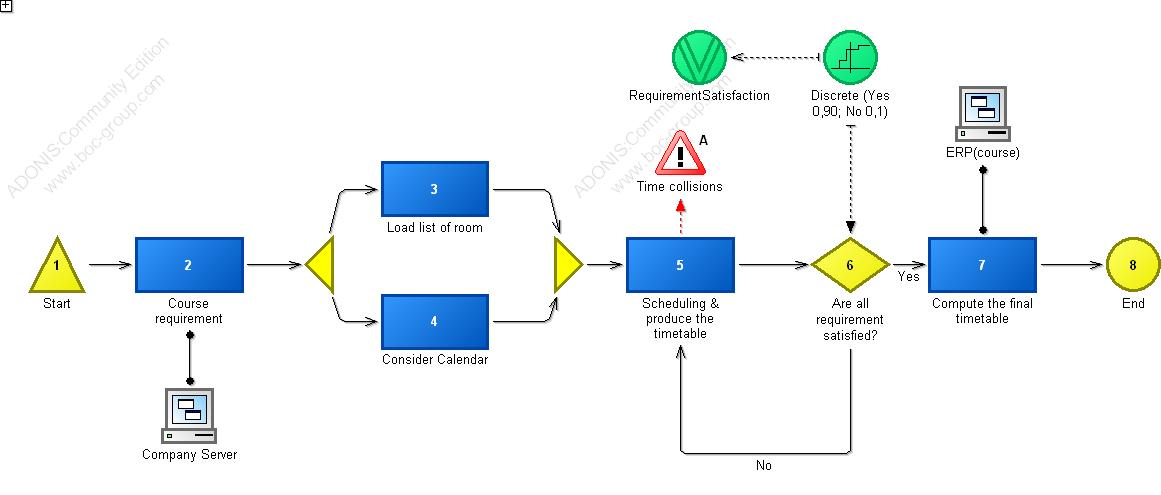
\includegraphics[scale=0.50,angle=90]{assign2/adonis/imgs/timetable.jpg}
\caption{Definition of the courses timetable}
\label{2img:timetable}
\end{figure}

\subsubsection{Path Analysis}


\begin{table}[ht!]
\centering
\begin{tabular}{|l|l|l|l|l|}
\hline
Path&Probability&Execution time&Cycle time&Costs\\
\hline
1&0,898000&00:000:00:47:00&00:000:00:46:00&9,000000\\
\hline
2&0,093000&00:000:00:57:00&00:000:00:56:00&9,500000\\
\hline
3&0,008000&00:000:01:07:00&00:000:01:06:00&10,000000\\
\hline
4&0,001000&00:000:01:17:00&00:000:01:16:00&10,500000\\
\hline
\end{tabular}
\end{table}

\begin{alltt}
Probability:   89,8000%
Execution time:  00:000:00:47:00
Waiting time:  00:000:00:00:00
Resting time:  00:000:00:00:00
Transport time:  00:000:00:00:00
Cycle time:  00:000:00:46:00
Costs:  9,000000

Timetable 0.1 (Business process model)
========================================
Process start: Start
Activity: Course requirement
Parallelity: Parallelity-33508
    *
    Activity: Load list of room
    *
    Activity: Consider Calendar
Merging: Merging-33536
Activity: Scheduling & produce the timetable
Decision: Are all requirement satisfied? --> RequirementSatisfaction='Yes'
Activity: Compute the final timetable
End: End
\end{alltt}

\subsubsection{Capacity Analysis}
The table \ref{2tab:timetab} shows the results of capacity analysis.

\begin{landscape}
\centering
\begin{table}
{\tiny
\begin{tabular}{|l|l|l|l|l|l|l|}
Business process&Activity&Performer&Number&Execution time&Cycle
time&Costs\\
\hline
Timetable 0.1&&&&00:000:00:48:01&00:000:00:47:01&9,051000\\
\hline
&Compute the final timetable &&1,000000&00:000:00:02:00&&0,100000\\
\hline
&&Secretary &1,000000&00:000:00:02:00&&0,100000\\
\hline
&Scheduling \& produce the timetable &&1,102000&00:000:00:11:01&&0,551000\\
\hline
&&Secretary &1,102000&00:000:00:11:01&&0,551000\\
\hline
&Load list of room &&1,000000&00:000:00:01:00&&0,100000\\
\hline
&&Secretary &1,000000&00:000:00:01:00&&0,100000\\
\hline
&Consider Calendar &&1,000000&00:000:00:04:00&&0,300000\\
\hline
&&Secretary &1,000000&00:000:00:04:00&&0,300000\\
\hline
&Course requirement &&1,000000&00:000:00:30:00&&8,000000\\
\hline
&&Secretary &1,000000&00:000:00:30:00&&8,000000\\
\hline
Total&&&&00:000:00:48:01&&9,051000\\
\hline
\end{tabular}
}
\caption{Scheduling of timetable, capacity analysis} 
\label{2tab:timetab}
\end{table}
\end{landscape}





\subsection{Course organization}
This process is one of the most important in this area, in fact it manages
the effective organization of a course. During this process the attention
is focused, on a firs phase on the teacher selection and the gathering of
course material and planning definition.

If needed the people selected for the teacher role can be trained on the
course methodologies. After this first phase, are preformed  some
activities regarding the definition of the courses structure, the presence
of practical lessons, possible correlation with other courses and the
examination details.

All these informations are then integrated and published. The structure of
this process can be seen in figure \ref{2img:course_organization}.

\begin{figure}[!ht]
\centering
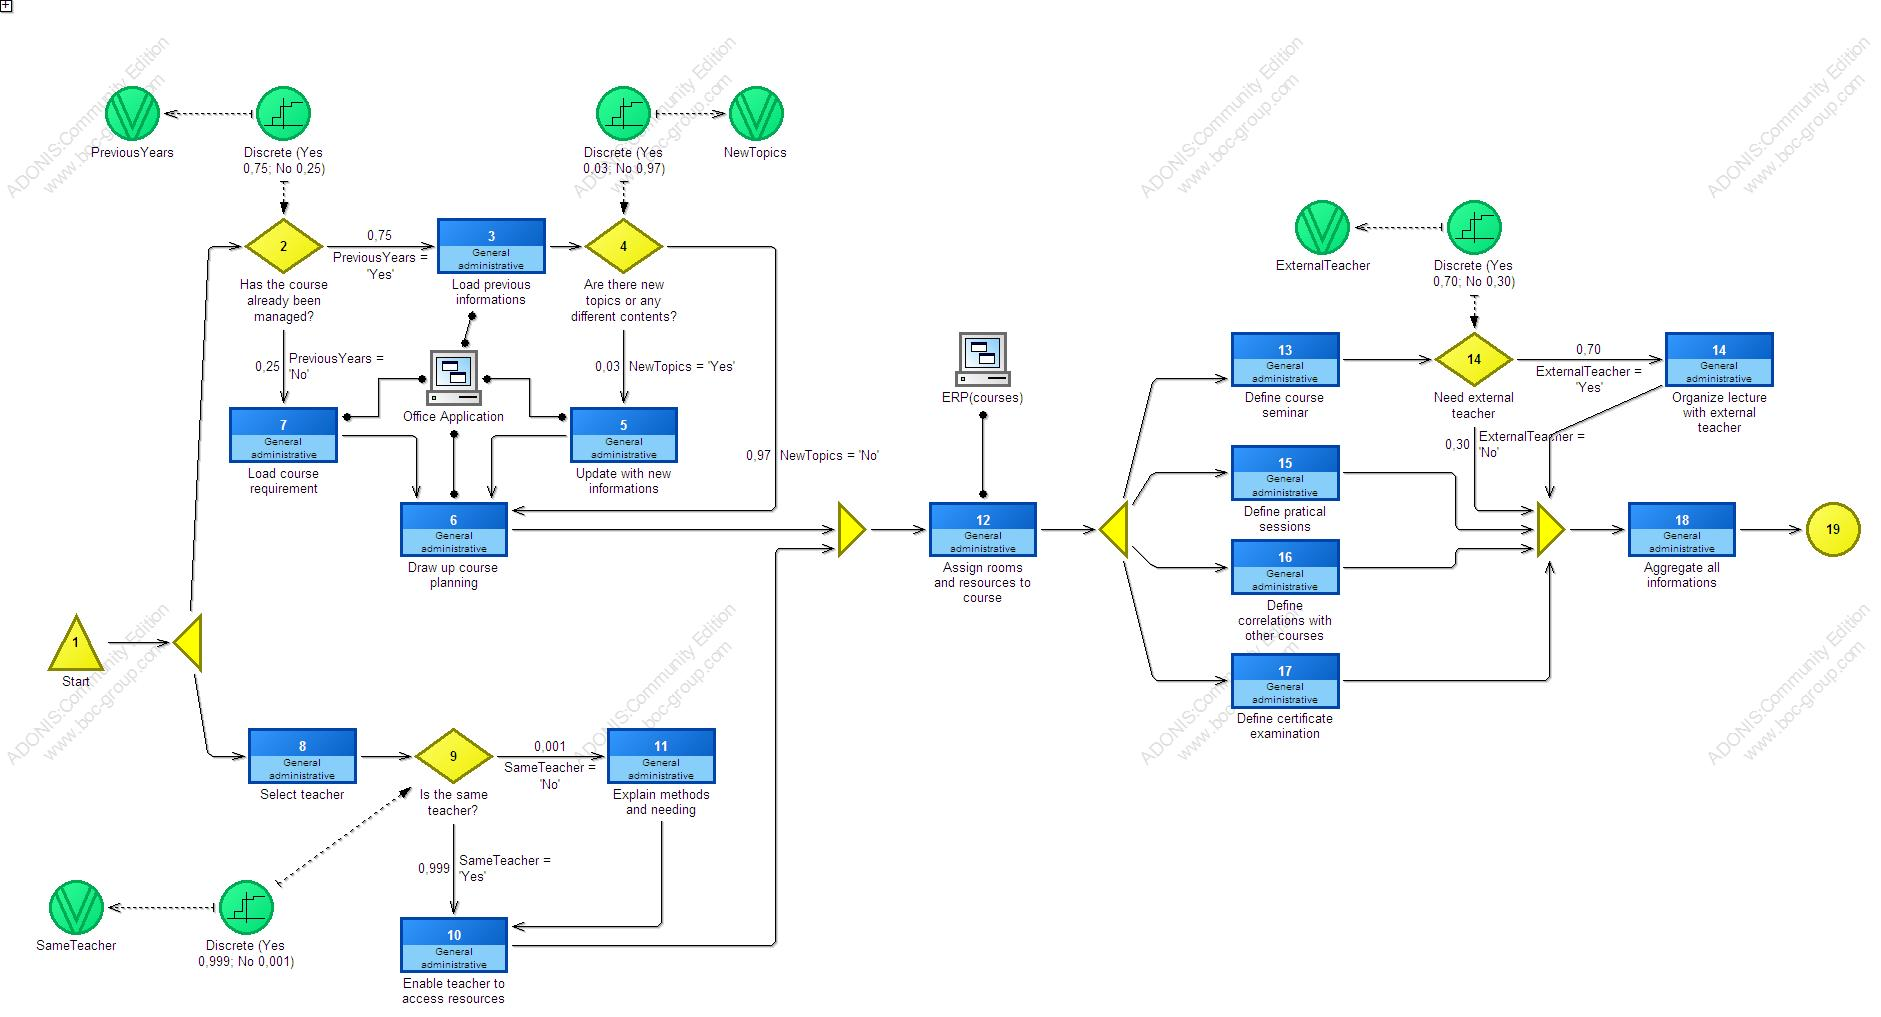
\includegraphics[scale=0.27, angle=90]{assign2/adonis/imgs/course_organization.jpg}
\caption{Organization of a formative course}
\label{2img:course_organization}
\end{figure}


\subsubsection{Path Analysis}

\begin{table}[ht!]
\centering
\begin{tabular}{|l|l|l|l|l|}
\hline
Path&Probability&Execution time&Cycle time&Costs\\
\hline
1&0,501000&00:000:05:15:00&00:000:03:41:00&418,500000\\
\hline
2&0,207000&00:000:03:15:00&00:000:01:41:00&168,500000\\
\hline
3&0,188000&00:000:05:15:00&00:000:03:41:00&418,600000\\
\hline
4&0,084000&00:000:03:15:00&00:000:01:41:00&168,600000\\
\hline
5&0,012000&00:000:06:15:00&00:000:04:34:00&438,500000\\
\hline
6&0,008000&00:000:04:15:00&00:000:02:34:00&188,500000\\
\hline
\end{tabular}
\end{table}

\begin{alltt}
Probability:   50,1000%
Execution time:  00:000:05:15:00
Waiting time:  00:000:00:00:00
Resting time:  00:000:00:00:00
Transport time:  00:000:00:00:00
Cycle time:  00:000:03:41:00
Costs:  418,500000

Course Organization 0.1 (Business process model)
========================================
Process start: Start
Parallelity: Parallelity-33578
    *
    Decision: Has the course already been managed? --> PreviousYears = 'Yes'
    Activity: Load previous informations
    Decision: Are there new topics or any different contents? --> NewTopics = 'No'
    Activity: Draw up course planning
    *
    Activity: Select teacher
    Decision: Is the same teacher? --> SameTeacher = 'Yes'
    Activity: Enable teacher to access resources
Merging: Merging-34785
Activity: Assign rooms and resources to course
Parallelity: Parallelity-34816
    *
    Activity: Define course seminar
    Decision: Need external teacher --> ExternalTeacher = 'Yes'
    Activity: Organize lecture with external teacher
    *
    Activity: Define pratical sessions
    *
    Activity: Define correlations with other courses
    *
    Activity: Define certificate examination
Merging: Merging-34835
Activity: Aggregate all informations
End: End-34847
\end{alltt}

\subsubsection{Capacity Analysis}
The table \ref{2tab:course_org} shows the results of capacity analysis.


\begin{landscape}
\centering
\begin{table}
{\tiny
\begin{tabular}{|l|l|l|l|l|l|l|}
Business process&Activity&Performer&Number&Execution time&Cycle
time&Costs\\
\hline
Course Organization 0.1&&&&00:000:04:40:44&00:000:03:06:35&344,737600\\
\hline
&Load previous informations &&0,724000&00:000:00:02:54&&0,217200\\
\hline
&&Secretary &0,724000&00:000:00:02:54&&0,217200\\
\hline
&Update with new informations &&0,023000&00:000:00:01:23&&0,460000\\
\hline
&&Secretary &0,023000&00:000:00:01:23&&0,460000\\
\hline
&Draw up course planning &&1,000000&00:000:00:40:00&&9,000000\\
\hline
&&Secretary &1,000000&00:000:00:40:00&&9,000000\\
\hline
&Load course requirement &&0,276000&00:000:00:01:06&&0,110400\\
\hline
&&Secretary &0,276000&00:000:00:01:06&&0,110400\\
\hline
&Enable teacher to access resources &&1,000000&00:000:00:01:00&&0,200000\\
\hline
&&Secretary &1,000000&00:000:00:01:00&&0,200000\\
\hline
&Assign rooms and resources to course &&1,000000&00:000:00:10:00&&1,000000\\
\hline
&&Secretary &1,000000&00:000:00:10:00&&1,000000\\
\hline
&Define course seminar &&1,000000&00:000:00:30:00&&30,000000\\
\hline
&&Secretary &1,000000&00:000:00:30:00&&30,000000\\
\hline
&Define pratical sessions &&1,000000&00:000:00:20:00&&3,000000\\
\hline
&&Secretary &1,000000&00:000:00:20:00&&3,000000\\
\hline
&Define correlations with other courses &&1,000000&00:000:00:10:00&&2,000000\\
\hline
&&Secretary &1,000000&00:000:00:10:00&&2,000000\\
\hline
&Define certificate examination &&1,000000&00:000:00:20:00&&2,000000\\
\hline
&&Secretary &1,000000&00:000:00:20:00&&2,000000\\
\hline
&Aggregate all informations &&1,000000&00:000:00:10:00&&1,000000\\
\hline
&&Secretary &1,000000&00:000:00:10:00&&1,000000\\
\hline
&Organize lecture with external teacher &&0,703000&00:000:01:24:22&&175,750000\\
\hline
&&Secretary &0,703000&00:000:01:24:22&&175,750000\\
\hline
&Select teacher &&1,000000&00:000:00:50:00&&120,000000\\
\hline
&&Secretary &1,000000&00:000:00:50:00&&120,000000\\
\hline
Total&&&&00:000:04:40:44&&344,737600\\
\hline
\end{tabular}
}
\caption{Capacity analysis for the process of organize a course} 
\label{2tab:course_org}
\end{table}
\end{landscape}




\subsection{Course Material Management}
This process, as in figure \ref{2img:course_material}, represents the way
in which AllSpark manages the material needed as support for a course.
Obviously in order to provide a right choice of material is necessary to
analyze deeply the course scope.

Other important things are the quality of the material offered and its
consistency, in terms of completeness and correctness. AllSpark uses its
own infrastructure in order to offer a sort of reliable repository of
course material and documentation. The access to this repository is
scheduled consistently with the course schedule.

\begin{figure}[!ht]
\centering
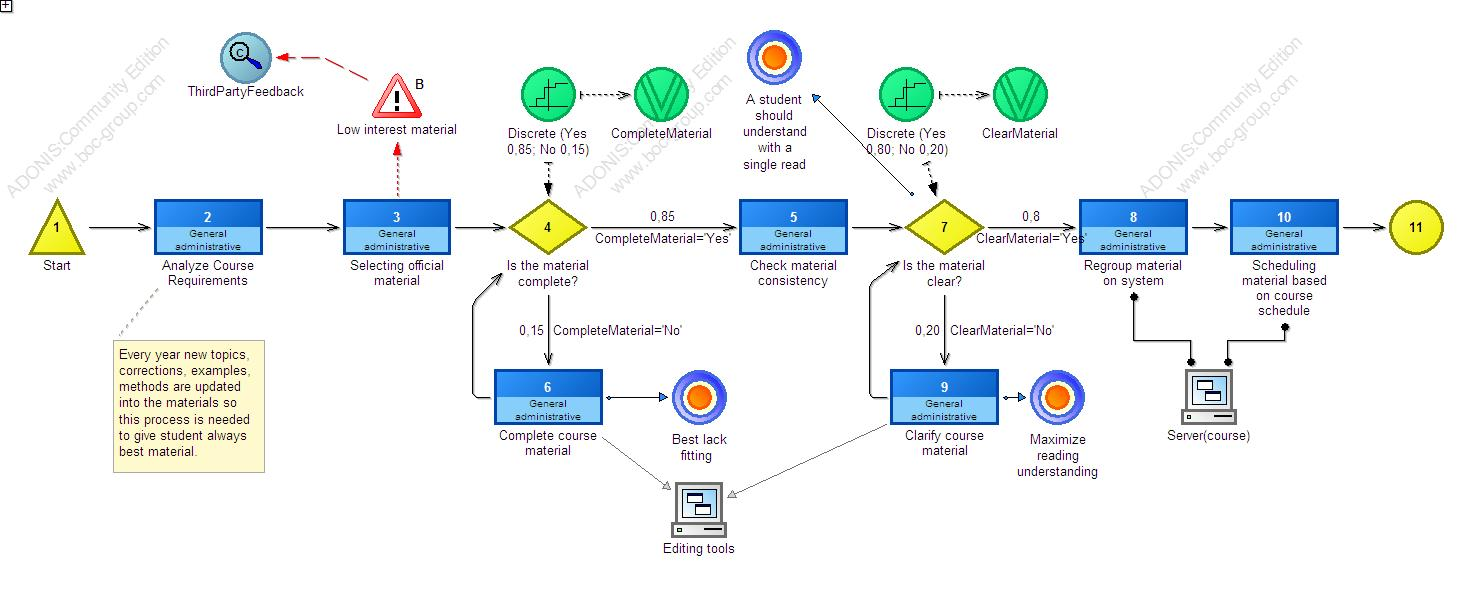
\includegraphics[scale=0.45, angle=90]{assign2/adonis/imgs/course_material.jpg}
\caption{Gathering and evaluation of course material}
\label{2img:course_material}
\end{figure}


\subsubsection{Path Analysis}

\begin{table}[ht!]
\centering
\begin{tabular}{|l|l|l|l|l|}
\hline
Path&Probability&Execution time&Cycle time&Costs\\
\hline
1&0,683000&00:000:02:20:00&00:000:02:20:00&51,500000\\
\hline
2&0,136000&00:000:02:40:00&00:000:02:40:00&60,500000\\
\hline
3&0,101000&00:000:02:40:00&00:000:02:40:00&61,500000\\
\hline
4&0,025000&00:000:03:00:00&00:000:03:00:00&70,500000\\
\hline
5&0,024000&00:000:03:00:00&00:000:03:00:00&69,500000\\
\hline
6&0,016000&00:000:03:00:00&00:000:03:00:00&71,500000\\
\hline
7&0,005000&00:000:03:20:00&00:000:03:20:00&78,500000\\
\hline
8&0,004000&00:000:03:20:00&00:000:03:20:00&80,500000\\
\hline
9&0,003000&00:000:03:20:00&00:000:03:20:00&81,500000\\
\hline
10&0,001000&00:000:04:20:00&00:000:04:20:00&107,500000\\
\hline
11&0,001000&00:000:03:20:00&00:000:03:20:00&79,500000\\
\hline
12&0,001000&00:000:04:00:00&00:000:04:00:00&96,500000\\
\hline
\end{tabular}
\end{table}

\begin{alltt}
Probability:   68,3000%
Execution time:  00:000:02:20:00
Waiting time:  00:000:00:00:00
Resting time:  00:000:00:00:00
Transport time:  00:000:00:00:00
Cycle time:  00:000:02:20:00
Costs:  51,500000

Course material 0.1 (Business process model)
========================================
Process start: Start
Activity: Analyze Course Requirements
Activity: Selecting official material
Decision: Is the material complete? --> CompleteMaterial='Yes'

Activity: Check material consistency
Decision: Is the material clear? --> ClearMaterial='Yes'
Activity: Regroup material on system
Activity: Scheduling material based on course schedule
End: End-35061
\end{alltt}

\subsubsection{Capacity Analysis}
The table \ref{2tab:material} shows the results of capacity analysis.

\begin{landscape}
\centering
\begin{table}
{\tiny
\begin{tabular}{|l|l|l|l|l|l|l|}
Business process&Activity&Performer&Number&Execution time&Cycle
time&Costs\\
\hline
Course material 0.1&&&&00:000:02:28:35&00:000:02:28:35&55,547000\\
\hline
&Analyze Course Requirements &&1,000000&00:000:00:15:00&&1,000000\\
\hline
&&Secretary &1,000000&00:000:00:15:00&&1,000000\\
\hline
&Selecting official material &&1,000000&00:000:01:00:00&&20,000000\\
\hline
&&Secretary &1,000000&00:000:01:00:00&&20,000000\\
\hline
&Check material consistency &&1,000000&00:000:01:00:00&&30,000000\\
\hline
&&Secretary &1,000000&00:000:01:00:00&&30,000000\\
\hline
&Scheduling material based on course schedule &&1,000000&00:000:00:02:00&&0,200000\\
\hline
&&Secretary &1,000000&00:000:00:02:00&&0,200000\\
\hline
&Regroup material on system &&1,000000&00:000:00:03:00&&0,300000\\
\hline
&&Secretary &1,000000&00:000:00:03:00&&0,300000\\
\hline
&Complete course material &&0,186000&00:000:00:03:43&&1,860000\\
\hline
&&Secretary &0,186000&00:000:00:03:43&&1,860000\\
\hline
&Clarify course material &&0,243000&00:000:00:04:52&&2,187000\\
\hline
&&Secretary &0,243000&00:000:00:04:52&&2,187000\\
\hline
Total&&&&00:000:02:28:35&&55,547000\\
\hline
\end{tabular}
}
\caption{Capacity analysis for the process of organizing course material} 
\label{2tab:material}
\end{table}
\end{landscape}




\subsection{Examinations}
At the end of the most of the courses, an official examination is planned,
this is very important in order to achieve the goal of gain renown as a
certification authority. In fact the AllSpark standard in this area is to
keep the level of the course and of the examination quite high, in order to
add an ulterior value to our certifications.

Often AllSpark provides examination service for other Authorities, in this
case is necessary to retrieve from them the original text and organize the
examination over that particular test.

Difficulties on this process can be originated by the ambiguos nature of
some examination modalities, like for example open questions, which can
lead to misjudgement and wrong results in the evaluation.
The process is described by figure \ref{2img:examination}.

\begin{figure}[!ht]
\centering
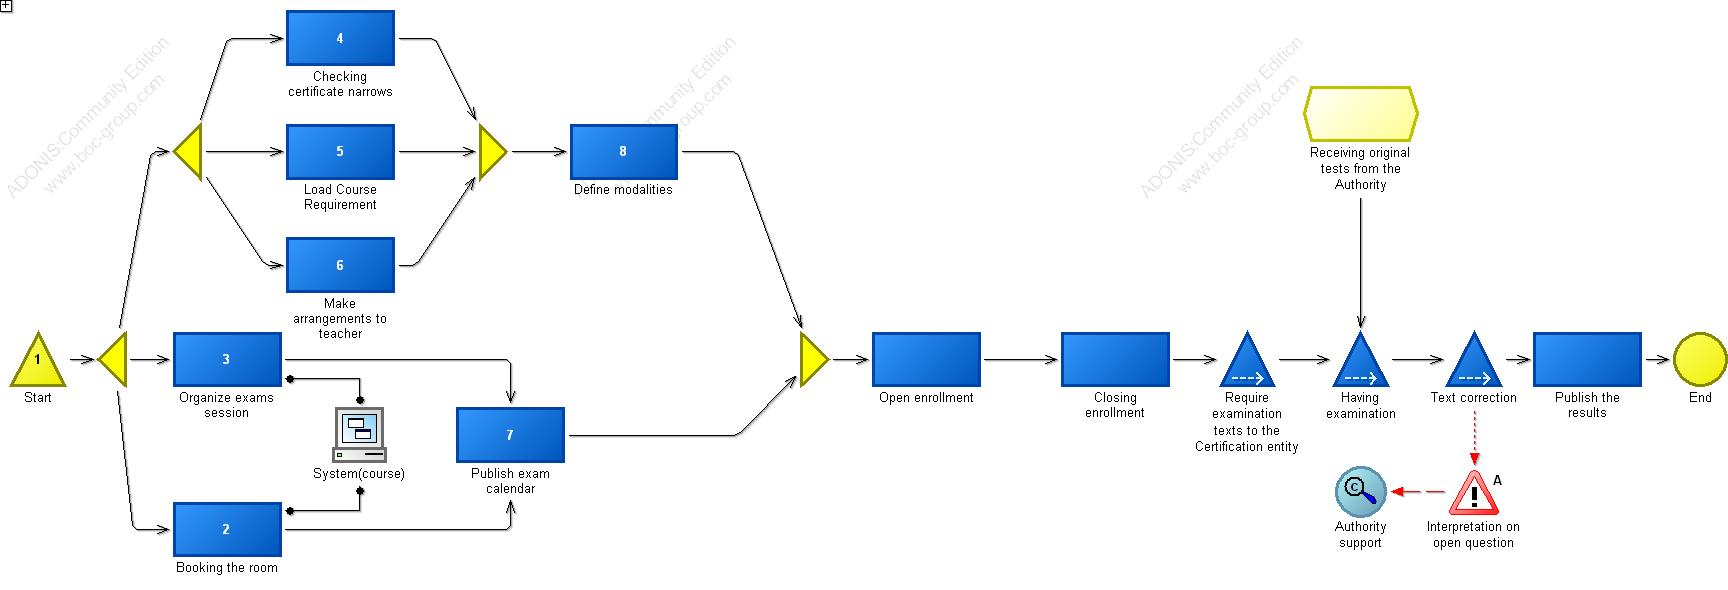
\includegraphics[scale=0.35, angle=90]{assign2/adonis/imgs/examination.jpg}
\caption{Organization of an examination test}
\label{2img:examination}
\end{figure}



\subsubsection{Path Analysis}

\begin{table}[ht!]
\centering
\begin{tabular}{|l|l|l|l|l|}
\hline
1&1,000000&00:001:01:57:00&00:001:01:31:00&94,100000\\
\hline
\end{tabular}
\end{table}

\begin{alltt}
Probability:   100,0000%
Execution time:  00:001:01:57:00
Waiting time:  00:000:00:00:00
Resting time:  00:000:00:00:00
Transport time:  00:000:00:00:00
Cycle time:  00:001:01:31:00
Costs:  94,100000

Examination 0.1 (Business process model)
========================================
Process start: Start
Parallelity: Parallelity-35109
    *
    Activity: Booking the room
    Activity: Publish exam calendar
    *
    Activity: Organize exams session
    Activity: Publish exam calendar
    *
    Parallelity: Parallelity-35154
        *
        Activity: Load Course Requirement
        *
        Activity: Checking certificate narrows
        *
        Activity: Make arrangements to teacher
    Merging: Merging-35157
    Activity: Define modalities
Merging: Merging-35174
Activity: Open enrollment
Activity: Closing enrollment
Activity: Require original test
Activity: Test correction
Activity: Publish the results
End: End
\end{alltt}

\subsubsection{Capacity Analysis}
The table \ref{2tab:exam} shows the results of capacity analysis.

\begin{landscape}
\centering
\begin{table}
{\tiny
\begin{tabular}{|l|l|l|l|l|l|l|}
Business process&Activity&Performer&Number&Execution time&Cycle
time&Costs\\
\hline
Examination 0.1&&&&00:001:01:57:00&00:001:01:31:00&94,100000\\
\hline
&Load Course Requirement &&1,000000&00:000:00:02:00&&0,200000\\
\hline
&&Secretary &1,000000&00:000:00:02:00&&0,200000\\
\hline
&Checking certificate narrows &&1,000000&00:000:00:10:00&&1,000000\\
\hline
&&Secretary &1,000000&00:000:00:10:00&&1,000000\\
\hline
&Booking the room &&1,000000&00:000:00:02:00&&0,100000\\
\hline
&&Secretary &1,000000&00:000:00:02:00&&0,100000\\
\hline
&Open enrollment &&1,000000&00:000:00:02:00&&0,700000\\
\hline
&&Secretary &1,000000&00:000:00:02:00&&0,700000\\
\hline
&Organize exams session &&1,000000&00:000:00:10:00&&0,800000\\
\hline
&&Secretary &1,000000&00:000:00:10:00&&0,800000\\
\hline
&Define modalities &&1,000000&00:000:00:30:00&&3,000000\\
\hline
&&Secretary &1,000000&00:000:00:30:00&&3,000000\\
\hline
&Make arrangements to teacher &&1,000000&00:000:00:10:00&&2,000000\\
\hline
&&Secretary &1,000000&00:000:00:10:00&&2,000000\\
\hline
&Publish exam calendar &&2,000000&00:000:00:02:00&&0,800000\\
\hline
&&Secretary &2,000000&00:000:00:02:00&&0,800000\\
\hline
&Closing enrollment &&1,000000&00:000:00:02:00&&0,300000\\
\hline
&&Secretary &1,000000&00:000:00:02:00&&0,300000\\
\hline
&Publish the results &&1,000000&00:000:00:02:00&&0,200000\\
\hline
&&Secretary &1,000000&00:000:00:02:00&&0,200000\\
\hline
&Require original test &&1,000000&00:000:00:45:00&&5,000000\\
\hline
&&Secretary &1,000000&00:000:00:45:00&&5,000000\\
\hline
&Test correction &&1,000000&00:001:00:00:00&&80,000000\\
\hline
&&Secretary &1,000000&00:001:00:00:00&&80,000000\\
\hline
Total&&&&00:001:01:57:00&&94,100000\\
\hline
\end{tabular}
}
\caption{Capacity analysis for the process of organize examination} 
\label{2tab:exam}
\end{table}
\end{landscape}




\subsection{Certification management}
This process permits to manage the delivery of the certification to the
candidates who passed the examination. Often the certification is provided
by an external organization, for which AllSpark acts as an examination
authority. In this case in necessary to send them the list of approved
candidates, and retrieve the certification documents.

This process can handle the case in which a single certification is
considered as a hierarchy of other certifications, in this case all the
other documents are equally retrieved.

The image in figure \ref{2img:certification} describes this process. Here
the final document is customized with AllSpark logo and information.

\begin{figure}[!ht]
\centering
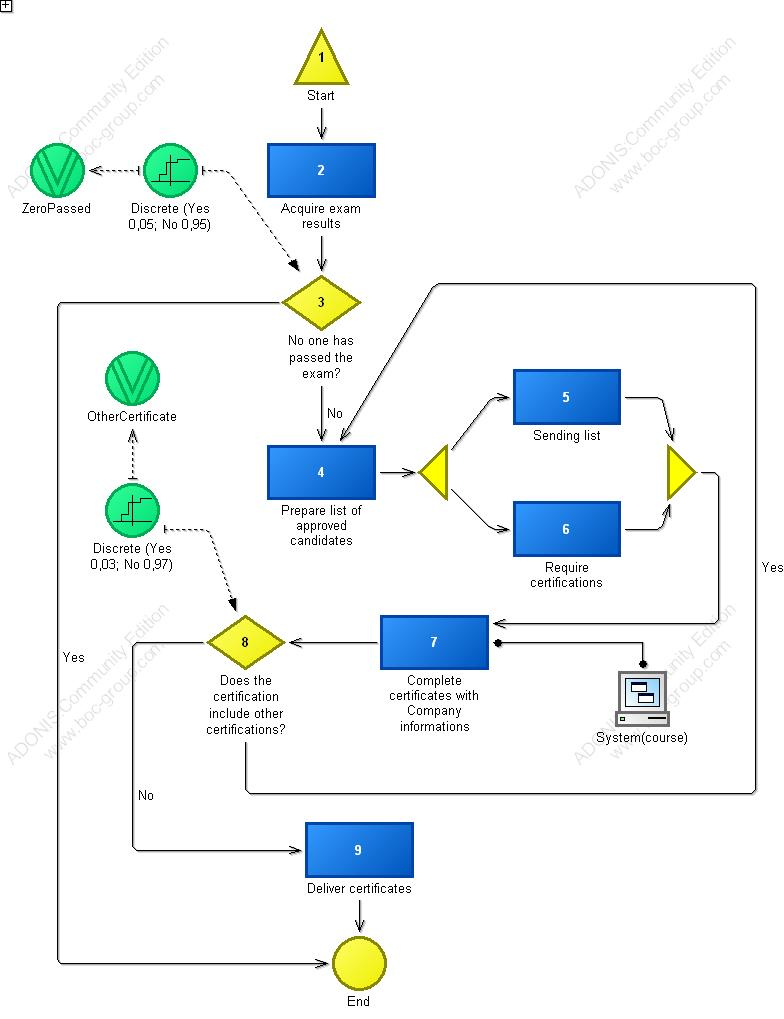
\includegraphics[scale=0.55]{assign2/adonis/imgs/certification.jpg}
\caption{Delivery of certification documents}
\label{2img:certification}
\end{figure}




\subsubsection{Path Analysis}

\begin{table}[ht!]
\centering
\begin{tabular}{|l|l|l|l|l|}
\hline
Path&Probability&Execution time&Cycle time&Costs\\
\hline
Path&Probability&Execution time&Cycle time&Costs\\
\hline
1&0,921000&00:000:00:54:00&00:000:00:49:00&13,700000\\
\hline
2&0,044000&00:000:00:02:00&00:000:00:02:00&0,100000\\
\hline
3&0,034000&00:000:01:41:00&00:000:01:31:00&26,400000\\
\hline
4&0,001000&00:000:02:28:00&00:000:02:13:00&39,100000\\
\hline
\end{tabular}
\end{table}

\begin{alltt}
Probability:   92,1000%
Execution time:  00:000:00:54:00
Waiting time:  00:000:00:00:00
Resting time:  00:000:00:00:00
Transport time:  00:000:00:00:00
Cycle time:  00:000:00:49:00
Costs:  13,700000

Certification 0.1 (Business process model)
========================================
Process start: Start
Activity: Acquire exam results
Decision: No one has passed the exam? --> ZeroPassed='No'
Activity: Prepare list of approved candidates
Parallelity: Parallelity-35259
    *
    Activity: Sending list
    *
    Activity: Require certifications
Merging: Merging-35265
Activity: Complete certificates with Company informations
Decision: Does the certification include other certifications? --> OtherCertificate='No'

Activity: Deliver certificates
End: End
\end{alltt}

\subsubsection{Capacity Analysis}
The table \ref{2tab:exam} shows the results of capacity analysis.

\begin{landscape}
\centering
\begin{table}
{\tiny
\begin{tabular}{|l|l|l|l|l|l|l|}
Business process&Activity&Performer&Number&Execution time&Cycle
time&Costs\\
\hline
Certification 0.1&&&&00:000:00:53:12&00:000:00:48:16&13,506200\\
\hline
&Acquire exam results &&1,000000&00:000:00:02:00&&0,100000\\
\hline
&&Secretary &1,000000&00:000:00:02:00&&0,100000\\
\hline
&Prepare list of approved candidates &&0,988000&00:000:00:01:59&&0,197600\\
\hline
&&Secretary &0,988000&00:000:00:01:59&&0,197600\\
\hline
&Sending list &&0,988000&00:000:00:04:56&&0,494000\\
\hline
&&Secretary &0,988000&00:000:00:04:56&&0,494000\\
\hline
&Require certifications &&0,988000&00:000:00:29:38&&2,964000\\
\hline
&&Secretary &0,988000&00:000:00:29:38&&2,964000\\
\hline
&Complete certificates with Company informations &&0,988000&00:000:00:09:53&&8,892000\\
\hline
&&Secretary &0,988000&00:000:00:09:53&&8,892000\\
\hline
&Deliver certificates &&0,954000&00:000:00:04:46&&0,858600\\
\hline
&&Secretary &0,954000&00:000:00:04:46&&0,858600\\
\hline
Total&&&&00:000:00:53:12&&13,506200\\
\hline
\end{tabular}
}
\caption{Capacity analysis for the process of delivering the certifications} 
\label{2tab:certs}
\end{table}
\end{landscape}


